\author{João Gonçalves}
\newcommand{\authorr}{Teresa Nogueira}
\newcommand{\studentID}{99995}
\newcommand{\studentIDD}{100029}
\newcommand{\supervisorone}{}
\newcommand{\supervisortwo}{}
\newcommand{\department}{Engenharia Eletrotécnica e de Computadores}
\newcommand{\exam}{Fundamentos de Energia Elétrica}

\title{%
Fundamentos de Energia Elétrica\\
Semana \#3 \& \#4\\
\large (Alguns tópicos \href{https://github.com/Kons-5}{\raisebox{0 em}{\large \faGithub}})}
\date{Setembro 2023}

\documentclass[a4paper, 10pt]{article}
\usepackage{packages}

%----------------------------------TITLE PAGE -----------------------------------
\makeatletter
\def\maketitle{
  \begin{center}\leavevmode
        \normalfont
        
\includegraphics[width=0.5\columnwidth]{img/title-page/IST.pdf}
        \vskip 0.05cm   
        \textsc{\large \department}\\
        \vskip 0.5cm
        \rule{0.95\linewidth}{0.2 mm} %\\
        {\large \exam}\\[0.5 cm]
        {\huge \bfseries \@title \par} 
        \vspace{1em}
        \begin{tikzpicture}
            \node[inner sep=6.66pt] (image) at (0,0) {
                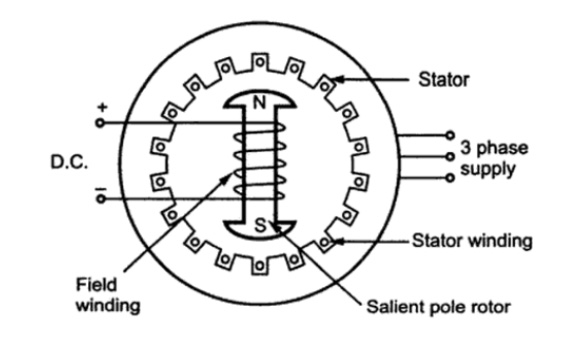
\includegraphics[scale=0.4]{img/title-page/000.jpg}
            };
            \draw[dashed] (image.south west) rectangle (image.north east);
        \end{tikzpicture}
        \vspace{-0.5em}
        \captionof*{figure}{\color{gray}Imagem: \textit{Máquina síncrona}}
        \vspace{0.5cm}
        \rule{0.95\linewidth}{0.2 mm} \\[0.75 cm]
        %\fontsize{9pt}{11pt}\selectfont
        \begin{minipage}[t]{\textwidth}
            \begin{flushleft} \large
                \emph{Autores:}\\
                \normalsize \textbf{\@author} : \studentID \\
                \fontsize{9pt}{11pt}\selectfont $\hookrightarrow$ jrazevedogoncalves@tecnico.ulisboa.pt \\
                \normalsize \textbf{\authorr} : \studentIDD \\
                \fontsize{9pt}{11pt}\selectfont $\hookrightarrow$ maria.teresa.ramos.nogueira@tecnico.ulisboa.pt
            \end{flushleft}
	   \end{minipage}%
    \vfill
	{\Large \@date\par}
   \end{center}
   %\vfill
   %\null
   \cleardoublepage
  }
\makeatother
%-------------------------------- ENDTITLE PAGE ----------------------------------

%---------------------------------- HEADER ------------------------------------
%\fancyhf{}
\renewcommand{\headrulewidth}{1pt}% Header rule width
\renewcommand{\footrulewidth}{0pt}% No footer rule
\setlength\headheight{26pt} 
\fancyhead[L]{\raisebox{0.1\height}[0pt][0pt]{\textit{Fundamentos de Energia Elétrica}}}
\fancyhead[R]{\raisebox{0.1\height}[0pt][0pt]{2023/2024}}
%-------------------------------- END HEADER ----------------------------------

\setcounter{tocdepth}{4}
\setcounter{secnumdepth}{4}
% \setcounter{secnumdepth}{-2}

\renewcommand{\figurename}{Fig.}
\renewcommand{\tablename}{Tab.}
\renewcommand{\contentsname}{Índice}
\settocbibname{\raisebox{0em}{Referências}}
\setlength{\bibsep}{0.15em}%reduzir espaço entre refs.

\pgfplotsset{compat=1.18}

\begin{document}
    \sloppy
    %% title page
    \pagenumbering{gobble}
    \maketitle
    
    %% toc
    \setcounter{tocdepth}{3}
    \tableofcontents
    \setcounter{tocdepth}{4}
    
    %% body
    \newpage
    \pagestyle{fancy}
    \pagenumbering{arabic}
    
    \setlength{\abovedisplayskip}{4pt}
    \setlength{\belowdisplayskip}{4pt}

    \clearpage
    \section{Conceitos Básicos}%
        %//==============================--@--==============================//%
\subsection{Energia e Potência. Diagrama de carga}
\label{subsec:energy-and-power}

A relação básica entre energia e potência exprime-se por:
$$
    P = \frac{dW}{dt} \qquad\rightleftarrows\qquad W = \int P\, dt
$$
onde $W$ denota a energia (expressa em joule, J) e $P$ a potência (expressa em watt, W).

\vspace{1em}
\noindent A carga de um Sistema de Energia Elétrica (SEE), varia significativamente ao longo do dia, acompanhando a atividade humana. Para um diagrama de carga define-se
$$
    h_d = \frac{W}{P_\text{max}}\, [\text{unidades de tempo}] \qquad\quad\qquad f_d = \frac{P_\text{med}}{P_\text{max}}\, [\%], \mkern9mu \text{em que } P_\text{med} = \frac{1}{T} \int_T P\, dt
$$
a \textit{utilização diária da ponta}, $h_d$, como a relação entre a energia e a potência máxima; e também o \textit{fator de carga diário}, $f_d$, como relação entre a potência média e a potência máxima.

\begin{figure}[H]
    \centering
    \scalebox{0.9}{%
        \begin{tikzpicture}
            \begin{axis}[
                xlabel={Horas}, xmin=0, xmax=24,
                xtick={0,2,4,6,8,10,12,14,16,18,20,22,24},
                ylabel={Carga $[$MW$]$}, ymin=0, ymax=50,
                ytick={0,5,10,15,20,25,30,35,40,45,50},
                grid=both,
                minor tick num=1,
                width=10cm,
                height=6.5cm
            ]
            
            \addplot [thick, line width=1.5pt, fill=gray!20, fill opacity=0.45] table [col sep=comma, x=Time, y=Load] {src/1/data.csv} \closedcycle;

            \addplot [mark=*, mark size=2pt, only marks] coordinates {(13, 41)};
            
            \node[above right, fill=white, fill opacity=0.6, text opacity=1, font=\large] at (13,41) {$P_\text{max}$};

            \node[above right, font=\large] at (10,10) {$W = \displaystyle \int P\, dt$};

            \draw [dashed, line width=1.25pt] (axis cs:0, 30.12) -- (axis cs:24, 30.12);

            \node[above, fill=white, fill opacity=0.6, text opacity=1, font=\large] at (4,30) {$P_\text{med}$};
            \end{axis}
        \end{tikzpicture}
    }
    \caption{Exemplo de diagrama de carga (diário)}
    \label{fig:diagrama-carga}
\end{figure}
%//==============================--@--==============================//%
\subsection{Potência em Sistemas de Energia Elétrica}
\label{subsec:power-SEE}

Os SEE atualmente funcionam quase na sua totalidade em corrente alternada --- com uma frequência de $50$ Hz na Europa e de $60$ Hz nos EUA e no Brasil ---, existindo casos especiais em que se utiliza a corrente contínua.\cite{paiva2005}

\renewcommand{\thefootnote}{\fnsymbol{footnote}}
\footnotetext[4]{%
    Em alguns países, como por exemplo no Japão, coexistem as duas frequências.
}
\renewcommand{\thefootnote}{\arabic{footnote}}

%//==============================--@--==============================//%
\subsubsection{Potência Instantânea, Potência Ativa e Reativa, Potência Complexa e Aparente}

Considerando um sistema monofásico constituído por um gerador que dá origem a uma tensão $v$ aos terminais de uma carga representada por uma impedância constante $Z$, define-se a \textit{potência instantânea} transferida do gerador para a carga como
$$
    \begin{aligned}
        p = v i &= \overbrace{\sqrt{2}V \cos(\omega t + \alpha_v)}^{\text{tensão }v} \cdot \overbrace{\sqrt{2}I \cos(\omega t + \alpha_i)}^{\text{corrente }i}, \qquad \forall (\alpha_v, \alpha_i) \in [0,2\pi] \times [0,2\pi]: \phi \in [-\pi/2,\pi/2] \\
        &= VI \cos(\phi) - VI \cos(2\omega t - \phi)
    \end{aligned}
$$
em que $\phi = \alpha_v - \alpha_i$ (desfasagem da tensão face à corrente). Massajando a expressão conclui-se
$$
    p = \underbrace{VI \cos(\phi) [1 - \cos(2 \omega t)]}_{p_1} - \underbrace{VI \sin(\phi) \sin(2\omega t)}_{p_2}
$$
Repare-se que a componente $p_1$ tem valor médio constante e $p_2$ tem valor médio nulo. A \textit{potência ativa} é o valor médio da potência instantânea, e corresponde portanto à potência efetivamente transferida:
$$
    P = VI \cos(\phi) \quad [\text{W}]
$$
A \textit{potência reativa} é o valor máximo da componente da potência que oscila entre o gerador e a carga, cujo valor médio é nulo, resultante da variação da energia magnética/elétrica armazenada nos elementos da carga:
$$
    Q = VI \sin(\phi) \quad [\text{VAr}]
$$
\noindent \textbf{Nota}: A grandeza $\cos(\phi)$ designa-se por \textit{fator de potência}, $fp \delequal P/S = \cos(\phi)$.

\clearpage
\vspace*{-2.25em}
\begin{centering}
    \begin{minipage}[b]{0.5\linewidth}
        \begin{figure}[H]
            \centering
            \scalebox{0.925}{%
            \begin{circuitikz}[scale=1.25]
                % Voltage source
                \draw (0,0) to[sV] (0,2.75) -- (4,2.75);
                % Arbitrary impedance (Z)
                \draw (4,2.75) node[circ] {} to[generic, l=$Z$, v=$v$] (4,0) node[circ] {}  -- (0,0);
                % Draw the current's arrow
                \draw[-latex, black, line width=0.9pt] (1.25,2.9) -- (2.75,2.9) node[midway,above] {$i$};
                % Label
                \draw (-0.35,0.7) node[xshift=0mm, yshift=2mm] {$(\omega)$};
            \end{circuitikz}}
            \caption{Sistema monofásico em corrente alternada}
        \end{figure}
    \end{minipage}%
    \begin{minipage}[b]{0.5\linewidth}
        \begin{figure}[H]
            \centering
            \scalebox{0.925}{%
            \begin{tikzpicture}[scale=1.25, >=latex]
                % Draw real and imaginary axes
                \draw[->] (-0.25,0) -- (2.5,0) node[right] {Re};
                \draw[->] (0,-0.25) -- (0,2.5) node[above] {Im};
                
                \draw [line width=1.25pt] (0,0) -- (2,0) -- (2,2) -- cycle;
        
                \draw [->, line width=1.25pt] (0,0) -- (2.025,2.025);
                
                \node[below] at (1,0) {$P$};
                \node[right] at (2,1) {$Q$};
                \node[above left] at (1,1) {$\mathbf{S}$};
                \node[right] at (2.2,2.4) {$|\mathbf{S}| = \sqrt{P^2 + Q^2} = VI$};
                \node[left] at (-1.15,2) {};

                \draw (0.75,0) arc (0:45:0.75); 
                \node[right] at (0.715,0.35) {$\phi$};
            \end{tikzpicture}}
            \caption{Representação das potências}
        \end{figure}
    \end{minipage}
\end{centering}

\noindent A \textit{potência complexa} é definida pelo produto do fasor tensão pelo conjugado do fasor corrente:
$$
    \mathbf{S} = \mathbf{V} \mathbf{I}^* = P + jQ \quad\text{em que}\quad
    \left\{\begin{aligned}
        \mathbf{V} &= V e^{j\alpha_v} \\
        \mathbf{I} &= I e^{j\alpha_i}
    \end{aligned}\right.
$$
A \textit{potência aparente} é definida como o módulo da potência complexa, i.e.,
$$
    S = |\mathbf{S}| = \sqrt{P^2 + Q^2} = VI \quad [\text{VA}]
$$
Além disto, a potência aparente representa a potência média ao longo do tempo para circuitos que se comportam como puramente resistivos ($\phi=0$).
%//==============================--@--==============================//%
\subsection{Sistema Elétrico Trifásico}

\noindent \textbf{Motivação}: A energia elétrica é produzida, transportada e distribuida em \textit{sistemas elétricos trifásicos}. A natureza pulsante da potência em sistemas monofásicos produz efeitos indesejaveis na operação dos sistemas elétricos. Nos motores elétricos, esta potência traduz-se num binário pulsante, por exemplo. A corrente trifásica elimina estas pulsações de potência e binário.

\begin{figure}[H]
    \centering
    \begin{circuitikz}[scale=0.625, transform shape]
        \draw (3.75,13.75) to[sinusoidal voltage source, sources/symbol/rotate=auto] (6.25,13.75);
        \draw (3.75,12.5) to[sinusoidal voltage source, sources/symbol/rotate=auto] (6.25,12.5);
        \draw (3.75,11.25) to[sinusoidal voltage source, sources/symbol/rotate=auto] (6.25,11.25);
        \draw [](3.75,13.75) to[short] (3.75,8.75);
        \draw [](6.25,13.75) to[short] (12.5,13.75);
        \draw [](6.25,12.5) to[short] (12.5,12.5);
        \draw [](6.25,11.25) to[short] (12.5,11.25);
        \draw (3.75,11.25) to[short, -*] (3.75,11.25);
        \draw (3.75,12.5) to[short, -*] (3.75,12.5);
        \draw (12.5,13.75) to[R, l=$Z$] (16.25,13.75);
        \draw (12.5,12.5) to[R, l=$Z$] (16.25,12.5);
        \draw (12.5,11.25) to[R, l=$Z$] (16.25,11.25);
        \draw [](16.25,13.75) to[short] (16.25,8.75);
        \draw (16.25,11.25) to[short, -*] (16.25,11.25);
        \draw (16.25,12.5) to[short, -*] (16.25,12.5);
        \draw [dashed] (2.5,8.75) -- (17.5,8.75);
        \draw [, dashed] (12.25,15) rectangle  (16.5,10);
        \draw [, dashed] (6.75,10) rectangle  (3.25,15);
        \draw (6.75,11.25) to[short, -*] (6.75,11.25);
        \draw (6.75,12.5) to[short, -*] (6.75,12.5);
        \draw (6.75,13.75) to[short, -*] (6.75,13.75);
        \draw (12.25,13.75) to[short, -*] (12.25,13.75);
        \draw (12.25,12.5) to[short, -*] (12.25,12.5);
        \draw (12.25,11.25) to[short, -*] (12.25,11.25);

        % Add overbrace and label
        \draw [decorate,decoration={brace,amplitude=5pt}] (3.25,15.15) -- (6.75,15.15) node[midway,above=12pt,font=\large] {Gerador trifásico};
        \draw [decorate,decoration={brace,amplitude=5pt}] (6.90,15.15) -- (12.10,15.15) node[midway,above=8pt,font=\large] {\parbox{3.85cm}{Linha de transmissão \\ trifásica}};
        \draw [decorate,decoration={brace,amplitude=5pt}] (12.25,15.15) -- (16.5,15.15) node[midway,above=10pt,font=\large] {Carga trifásica};

        % Label
        \draw (3.75,10.25) node[xshift=2.5cm, yshift=1.5mm] {$(\omega)$};
    \end{circuitikz}
    \caption{Sistema trifásico simétrico}
\end{figure}

%//==============================--@--==============================//%
\subsubsection{Tensão e Corrente}

\noindent Um gerador trifásico com os 3 enrolamentos em estrela produz 3 forças eletromotizes com frequência angular $w =2\pi f$, desfasados $\pm 2\pi/3 (= \pm 120^\degree)$. A fase de referência, possui argumento nulo.


\vspace{-0.5em}
\begin{centering}
    \begin{minipage}[b]{0.5\linewidth}
        \begin{figure}[H]
        \centering
            \scalebox{0.925}{%
            \begin{tikzpicture}[scale=0.825]
                \begin{axis}[
                domain=0:1, 
                samples=400, 
                axis lines=middle, 
                axis line style={-}, 
                xtick=\empty, 
                ytick=\empty, 
                xticklabel=\empty, 
                yticklabel=\empty,
                ymax = 1.15,
                xmax = 1.1,
                ]
                
                \addplot[black,thick] {sin(deg(2*pi*x))}; 
                \addplot[black,thick] {sin(deg(2*pi*x - 2*pi/3))}; 
                \addplot[black,thick] {sin(deg(2*pi*x + 2*pi/3))}; 
                
                \draw[dashed] (axis cs:1,1) -- (axis cs:1,-1); 
                \node at (axis cs:1.05,-0.1) {$2\pi$};
                \node at (axis cs:0.25,1.1) {$e_a$};
                \node at (axis cs:0.58,1.1) {$e_b$};
                \node at (axis cs:0.91,1.1) {$e_b$};
             \end{axis}
        \end{tikzpicture}}
        \caption{Variação no tempo das f.e.m}
    \end{figure}
    \end{minipage}%
    \begin{minipage}[b]{0.5\linewidth}
        \begin{figure}[H]
        \centering
            \scalebox{0.925}{%
            \begin{tikzpicture}[scale=1.25,>=stealth]
                 \coordinate (O) at (0,0);
        
                  \draw[->,thick] (O) -- ++(240:2cm) node[right] {$E_b$}; 
                  \draw[->,thick] (O) -- ++(360:2cm) node[below] {$E_a$}; 
                  \draw[->,thick] (O) -- ++(480:2cm) node[left] {$E_c$};
                
                  \draw[->, thick] (240:0.3cm) arc (240:360:0.3cm) node[midway, below] {$\frac{2\pi}{3}$};   
                  \draw[->, thick] (360:0.3cm) arc (360:480:0.3cm) node[midway, above] {$\frac{2\pi}{3}$};
                  \draw[->,thick] (480:0.3cm) arc (480:600:0.3cm) node[midway, left] {$\frac{2\pi}{3}$};
            \end{tikzpicture}}
        \caption{Diagrama de fasores}
        \end{figure}
    \end{minipage}
\end{centering}

%% next page
\clearpage
\begin{minipage}[c]{0.4\textwidth}
    \begin{figure}[H]
        \centering
        \begin{tikzpicture}[scale=1.5,>=stealth]
            \coordinate (O) at (0,0);
            
            \draw[->,thick] (O) -- ++(240:2cm) node[below] {$V_b$}; 
            \draw[->,thick] (O) -- ++(360:2cm) node[right] {$V_a$}; 
            \draw[->,thick] (O) -- ++(480:2cm) node[above] {$V_c$};
    
            \draw[->,thick] (O) -- ++(210:0.75cm) node[above] {$I_b$};
            \draw[->,thick] (O) -- ++(330:0.75cm) node[below] {$I_a$};
            \draw[->,thick] (O) -- ++(450:0.75cm) node[right] {$I_c$};
    
            \draw (360:0.3cm) arc (360:330:0.3cm) node[midway, right, below=, font=\small] {$\phi$};
            \draw (240:0.3cm) arc (240:210:0.3cm) node[midway, left, font=\small] {$\phi$};
            \draw (480:0.3cm) arc (480:450:0.3cm) node[midway, above, font=\small] {$\phi$};
    
            % Calculate the coordinates of the tips of V_a, V_b, and V_c
            \coordinate (tipA) at ($(O)+(360:2cm)$);
            \coordinate (tipB) at ($(O)+(240:2cm)$);
            \coordinate (tipC) at ($(O)+(480:2cm)$);
            
            % Draw vectors V_ab, V_ca, and V_bc
            \draw[->,thick,dashed] (tipB) -- (tipA) node[midway, below=0.75mm] {$V_{ab}$};
            \draw[->,thick,dashed] (tipA) -- (tipC) node[midway, above] {$V_{ca}$};
            \draw[->,thick,dashed] (tipC) -- (tipB) node[midway, left] {$V_{bc}$};
    
            % Draw the angle 
            \draw (O) ++(360:1.45cm) arc (180:210:0.55cm);
            \node at ($(O)+(351:1.3cm)$) {$\frac{\pi}{6}$};
        \end{tikzpicture}
        \caption{Fasores de tensão (simples e composta) e fasores de corrente num sistema trifásico simétrico.}
    \end{figure}
\end{minipage} \hfill
\begin{minipage}[c]{0.525\textwidth} \small
    \noindent As \textit{tensões simples} ou \textit{fase-neutro} são então: 
    $$ 
    \begin{aligned} 
        v_a &= \sqrt{2} V \sin(\omega t) \\ 
        v_b &= \sqrt{2} V \sin(\omega t - 2\pi/3) \\ 
        v_c &= \sqrt{2} V \sin(\omega t + 2\pi/3) 
    \end{aligned} 
    \qquad\rightleftarrows\qquad 
    \begin{aligned} 
        \mathbf{V}_{a} &= V e^{j0} \\ 
        \mathbf{V}_{b} &= V e^{-j2\pi/3} \\ 
        \mathbf{V}_{c} &= V e^{j2\pi/3} 
    \end{aligned} 
    $$ 
    
    Num sistema trifásico, define-se o valor das \textit{tensões fase-fase} (ou \textit{tensões entre fases} ou \textit{tensões compostas}): 
    $$ 
    \begin{aligned} 
        \mathbf{V}_{ab} &= \mathbf{V}_a - \mathbf{V}_b \\ 
        \mathbf{V}_{bc} &= \mathbf{V}_b - \mathbf{V}_c \\ 
        \mathbf{V}_{ca} &= \mathbf{V}_c - \mathbf{V}_a 
    \end{aligned} 
    \;\rightarrow\; 
    \boxed{\begin{aligned} 
        V_L &= V_{ab} = V_{bc} = V_{ca} = 2V \cos(\pi/6) \\ 
            &= \sqrt{3} V \mkern9mu\text{\small (valor eficaz das compostas)}
    \end{aligned}} 
    $$ 
    
    \noindent Uma vez que a carga é simétrica, as correntes escrevem-se: 
    $$ \begin{aligned} 
        i_a &= \sqrt{2} I \sin(\omega t - \phi) \\ 
        i_b &= \sqrt{2} I \sin(\omega t - \phi - 2\pi/3) \\ 
        i_c &= \sqrt{2} I \sin(\omega t - \phi + 2\pi/3) 
    \end{aligned} 
    \qquad\rightleftarrows\qquad 
    \begin{aligned} 
        \mathbf{I}_{a} &= I e^{-j\phi} \\ 
        \mathbf{I}_{b} &= I e^{-j(2\pi/3 + \phi)} \\ 
        \mathbf{I}_{c} &= I e^{j(2\pi/3 - \phi)} 
    \end{aligned} 
    $$
\end{minipage}

\begin{mdframed} % miminhos
    \noindent \textbf{Notas}:
    \begin{enumerate}[noitemsep,nolistsep,leftmargin=*,label=\arabic*.,font=\small\bfseries]\small
        \item ``A soma das correntes nas três fases é nula, logo não é necessário um condutor a conectar o neutro do gerador com o da carga. Os dois neutros estão ao potencial da terra, quer no gerador quer na carga.''\cite{paiva2005}
        
        \item ``Num sistema trifásico simétrico, todas as tensões simples podem ser medidas em relação a um neutro, que tem o mesmo potencial (zero) ao longo de todo o sistema.''\cite{paiva2005}
    \end{enumerate}
\end{mdframed}

%//==============================--@--==============================//%
\subsubsection{Potência Instantânea, Potência Ativa e Reativa, e Potência Complexa}

A potência transferida do gerador para a carga será a soma das potências instantâneas por fase:
$$
    p = v_a i_a + v_b i_b + v_c i_c = 3 VI \cos(\phi)
$$
Verifica-se que a \textit{potência trifásica instantânea} é constante, e igual a 3 vezes a potência ativa por fase.

Deste modo, a \textit{potência ativa trifásica} escreve-se:
$$
    P = 3 VI \cos(\phi) = \sqrt{3} V_L I \cos (\phi) \quad [\text{W}]
$$
A \textit{potência reativa trifásica} é definida como a soma algébrica das potências reativas em cada fase:
$$
    Q = 3 VI \sin(\phi) = \sqrt{3} V_L I \sin (\phi) \quad [\text{VAr}]
$$
A \textit{potências complexa e aparente para sistemas trifásicos} é dada por:
$$
\begin{aligned}
    \mathbf{S} &= 3\mathbf{V} \mathbf{I}^* = P + jQ\\
    S &= \sqrt{P^2 + Q^2} = 3VI = \sqrt{3} V_L I \quad [\text{VA}]
\end{aligned}
$$

%//==============================--@--==============================//%
\subsubsection{Carga Ligada em Triângulo}

\noindent Outra forma de ligar a carga é em \underline{triângulo}, situação em que cada impedância de carga \textbf{Z} está sujeita à tensão entre fases.

\begin{centering}
    \begin{minipage}[b]{0.4\linewidth}
        \begin{figure}[H]
        \centering
        \resizebox{0.75\textwidth}{!}{%
        \begin{circuitikz}[>=stealth]
        % Nodes
        \draw (-2,2) to[short, -*] (-2,2);
        \draw (-2,0) to[short, -*] (-2,0);
        \draw (-2,-2) to[short, -*] (-2,-2);
        
        %Lines
        \draw [](-2,0) to[short] (1,0);
        \draw (1,0) to[short, -*] (1,0);
        \draw (1,0) to[R,*-*] (2.5,2);
        \draw (1,0) to[R,*-*] (2.5,-2);
        \draw (2.5,2) to[R,*-*] (2.5,-2);
        \draw (-2,2) to[short, -*] (2.5,2);
        \draw (-2,-2) to[short, -*] (2.5,-2);
        
        \node at (3,0) {$Z_\Delta$};
        \node at (1.1,1) {$Z_\Delta$};
        \node at (1.1,-1) {$Z_\Delta$};
        
        \node[coordinate,label=left:$a$] at (-2,2) {};
        \node[coordinate,label=left:$b$] at (-2,0) {};
        \node[coordinate,label=left:$c$] at (-2,-2) {};
        
        % Arrows
        \draw[->,thick](-2, 1.8) to[short] (-2,0.2);
        \draw[->,thick](-2, -0.2) to[short] (-2,-1.8);
        \draw[->,thick](-2.5, -1.8) to[short] (-2.5,1.8);
        
        \node at (-2.9,0) {$V_{ca}$};
        \node at (-1.7,1) {$V_{ab}$};
        \node at (-1.7,-1) {$V_{bc}$};
        
        \draw[->,thick](0, 2) to[short] (0.1,2) node[above] {$I_a$};
        \draw[->,thick](0, 0) to[short] (0.1,0) node[above] {$I_b$};
        \draw[->,thick](0, -2) to[short] (0.1,-2) node[above] {$I_c$};
        
        \draw[->,thick](2.5, -1.5) to[short] (2.5,-1.3) node[right=0.1] {$I_{ca}$};
        
        
        \end{circuitikz}
        }%
        \caption{Carga ligada em triângulo.}
        \end{figure}
\end{minipage}%
    \begin{minipage}[b]{0.6\linewidth}
        \begin{mdframed}
            \noindent As correntes $\bar{I}_{ab}$, $\bar{I}_{bc}$ e $\bar{I}_{ca}$ são:
            \vspace{0.5em}
            $$
                \bar{I}_{ab} = \dfrac{\overline{V}_{ab}}{\overline{Z}_\Delta}\quad
                \bar{I}_{bc} = \dfrac{\overline{V}_{bc}}{\overline{Z}_\Delta}\quad
                \bar{I}_{ac} = \dfrac{\overline{V}_{ac}}{\overline{Z}_\Delta}
            $$
            \vspace{0.5em}
            \noindent A corrente na linha $I_a$ é, por conseguinte:
            $$
                \boxed{\bar{I}_a = \dfrac{\overline{V}_{ab} - \overline{V}_{ca}}{\overline{Z}_\Delta} = \dfrac{3\overline{V}_a}{\overline{Z}_\Delta}}
            $$
            \noindent A amplitude da corrente é \textbf{3 vezes maior} que na ligação da carga em estrela.
        \end{mdframed}
    \end{minipage}
\end{centering}

\noindent A \underline{potência absorvida} pela carga ligada em triângulo é \textbf{3 vezes maior} que a ligada em estrela, para o mesmo valor de impedância de carga.

%//==============================--@--==============================//%
\paragraph{Conversão entre Ligação em Estrela e Ligação em Triângulo (wye $\rightleftarrows$ delta)}

\begin{table}[ht]
    \centering
    \caption{Transformações Y-$\Delta$ e $\Delta$-Y}

    \setlength{\tabcolsep}{1cm}
    
    \begin{tabular}{cc}
        \begin{circuitikz}
            \ctikzset{resistors/scale=0.75}
            
            % Define interest points
            \coordinate (A) at (0,0);
            \coordinate (B) at (4,0);
            \coordinate (C) at (2,{-2*sqrt(3)});
            \coordinate (G) at (2,{-(2/3)*sqrt(3)});
    
            % Draw the skeleton
            \draw[dashed] (A) -- (G) -- (B);
            \draw[dashed] (G) -- (C);
    
            \node[circ] at (A) {};
            \node[circ] at (B) {};
            \node[circ] at (C) {};
            \node[circ] at (G) {};

            \node[left] at (A) {$a$};
            \node[right] at (B) {$b$};
            \node[below] at (C) {$c$};
    
            % Draw the impedances
            \draw (A) to[R, a=$Z_{ab}$] (B) to[R, a=$Z_{bc}$] (C) to[R, a=$Z_{ca}$] (A);
        \end{circuitikz}
        &
        \begin{circuitikz}
            \ctikzset{resistors/scale=0.75}
            
            % Define interest points
            \coordinate (A) at (0,0);
            \coordinate (B) at (4,0);
            \coordinate (C) at (2,{-2*sqrt(3)});
            \coordinate (G) at (2,{-(2/3)*sqrt(3)});
    
            % Draw the skeleton
            \draw[dashed] (A) -- (B) -- (C) -- (A);
            \node[circ] at (A) {};
            \node[circ] at (B) {};
            \node[circ] at (C) {};
            \node[circ] at (G) {};

            \node[left] at (A) {$a$};
            \node[right] at (B) {$b$};
            \node[below] at (C) {$c$};
            
            % Draw the impedances
            \draw (A) to[R, l=$Z_{a}$] (G) to[R, l=$Z_{b}$] (B);
            \draw (C) to[R, l=$Z_{c}$] (G);
        \end{circuitikz} \\
        $\begin{aligned}
            \boxed{\textbf{Y} \to \mathbf{\Delta}}\\
            Z_{ab} &= \frac{Z_aZ_b+Z_bZ_c+Z_cZ_a}{Z_c} \\
            Z_{bc} &= \frac{Z_aZ_b+Z_bZ_c+Z_cZ_a}{Z_a} \\
            Z_{ca} &= \frac{Z_aZ_b+Z_bZ_c+Z_cZ_a}{Z_b}
        \end{aligned}$
        & 
        $\begin{aligned}
            \boxed{\mathbf{\Delta} \to \textbf{Y}}\\
            Z_a &= \frac{Z_{ab}Z_{ca}}{Z_{ab}+Z_{bc}+Z_{ca}} \\
            Z_b &= \frac{Z_{bc}Z_{ab}}{Z_{ab}+Z_{bc}+Z_{ca}} \\
            Z_c &= \frac{Z_{ca}Z_{cb}}{Z_{ab}+Z_{bc}+Z_{ca}}
        \end{aligned}$ 
    \end{tabular}
\end{table}

%//==============================--@--==============================//%
\vspace*{-1em}%
\subsection{Valores por Unidade}

O uso de \textit{valores por unidade} (p.u.) consiste na quantificação das grandezas elétricas como frações de valores de base, designados por valores nominais ou de plena carga. O valor p.u. de uma grandeza obtém-se por
$$
    \text{valor p.u.} = \frac{\text{valor da grandeza}}{\text{valor da base}}
$$
\textbf{Nota}: O valor da grandeza pode ser um fasor/número complexo ou um valor instantâneo em unidades SI, enquanto o valor de base é um número real adequado. O valor de base pode ser \underline{postulado} ou \underline{derivado}.

%//==============================--@--==============================//%
\subsubsection{Sistemas Monofásicos}

\begin{mdframed}
    \noindent Num sistema monofásico, postula-se: 
    \begin{center}
        a \textit{base de tensão} $[$kV$]$, $V_b$ e a \textit{base de potência} $[$MVA$]$, $S_b$
    \end{center}
    \noindent Os valores de base derivados são:
    \begin{itemize}[noitemsep,label=-,font=\bfseries]
        \item \textit{base de corrente} $[$kA$]$, $$ I_b = S_b/V_b $$
        \item \textit{base de impedância} $[\Omega]$, $$ Z_b = V_b/I_b = V^2_b/S_b $$
        \item \textit{base de admitância} $[$S$]$, $$ Y_b = I_b/V_b = S_b/V^2_b$$
    \end{itemize}
\end{mdframed}

%//==============================--@--==============================//%
\subsubsection{Sistemas Trifásicos}

\begin{mdframed}
Analogamente, postula-se para base a tensão \underline{entre fases}, $V_b$, e a potência aparente \underline{trifásica}, $S_b$.

\vspace{1em}
\noindent Temos a relação $S_b = \sqrt{3} V_b I_b$, de onde se derivam as restantes:
\begin{itemize}[noitemsep,label=-,font=\bfseries]
        \item \textit{base de corrente} $[$kA$]$, $$ I_b = S_b/\sqrt{3}V_b $$
        \item \textit{base de impedância} $[\Omega]$, $$ Z_b = V_b/\sqrt{3}I_b = V^2_b/S_b $$
        \item \textit{base de admitância} $[$S$]$, $$ Y_b = \sqrt{3}I_b/V_b = S_b/V^2_b$$
    \end{itemize}
\end{mdframed}

%//==============================--@--==============================//%
\subsection{Transmissão de Energia}
\subsubsection{Corrente Alternada}
Considerando uma linha de transmissão de energia modelada por um elemento indutivo com reatância $X_L$, pretende-se estabelecer a relação entre as potências ativa e reativa que transitam na linha e as tensões nos nós entre as quais ela está ligada.

\vspace{-0.5em}
\begin{centering}
    \begin{minipage}[b]{0.5\linewidth}
        \begin{figure}[H]
        \centering
        \resizebox{0.8\textwidth}{!}{%
        \begin{circuitikz}[>=stealth]
        
        % Inductor
        \draw (0,0) to[cute inductor] (3,0);
        \node at (1.5,0.4) {$j X_L$};
        
        % Nodes
        \draw (0, 0) to[short, -*] (0,0);
        \draw (3,0) to[short, -*] (3,0);
        \draw (0,-2) to[short, -*] (0,-2);
        \draw (3,-2) to[short, -*] (3,-2);
        
        % Wire
        \draw (0, -2) to[short, -*] (3,-2);
        
        % Arrows
        \draw[->,thick](0, -0.2) to[short] (0,-1.8);
        \node at (-0.3,-1) {$V_1$};
        
        \draw[->,thick](3, -0.2) to[short] (3,-1.8);
        \node at (3.3,-1) {$V_2$};
        
        \draw[->,thick](0.5, 0) to[short] (0.55,0) node[above] {$I$};
        
        \end{circuitikz}
        }%
        \caption{Transmissão de energia --- elemento indutivo.}
        \end{figure}
\end{minipage}%
    \begin{minipage}[b]{0.5\linewidth}
        \begin{mdframed}
            A corrente que percorre a linha, definida como positiva no sentido $1 \rightarrow 2$:
            $$
                I = \dfrac{V_1 - V_2}{j X_L}
            $$
            A potência complexa $\mathbf{S}_{12}$:
            $$
            \begin{aligned}
                &\mathbf{S}_{12} = \mathbf{V_1} \mathbf{I^*} = \mathbf{V_1}\dfrac{ \mathbf{V}_1^* -  \mathbf{V}_2^*}{-j X_L} =\\ &\dfrac{ V_1^2 - \mathbf{V}_1\mathbf{V}_2^*}{-j X_L}\quad\text{em que}\quad
                \left\{\begin{aligned}
                    \mathbf{V}_1 &= V_1 e^{j\theta_1} \\
                    \mathbf{V}_2 &= V_2 e^{j\theta_2}
                \end{aligned}\right.
            \end{aligned}
            $$
        \end{mdframed}
    \end{minipage}
\end{centering}

\noindent Seja $\theta = \theta_1 - \theta_2$ o ângulo de desfasagem entre as tensões no nó 1 e no nó 2:
$$
\mathbf{S_{12}} = j\dfrac{ V_1^2 -  V_1 V_2 e^{j\theta}}{X_L} = \underbrace{\dfrac{V_1 V_2 \sin(\theta)}{X_L}}_{P_{12}} + \underbrace{j \dfrac{V_1^2 - V_1 V_2 \cos(\theta)}{X_L}}_{Q_{12}}
$$
De forma análoga se deduzem as potência ativa e reativa na receção, positivas no sentido $2 \rightarrow 1$:
$$
P_{21} = - \dfrac{V_1 V_2 \sin(\theta)}{X_L}\qquad 
Q_{21} = \dfrac{V_2^2 - V_1 V_2 \cos(\theta)}{X_L}
$$
Somando as duas equações vem que:
$$
\begin{aligned}
    &P_L = P_{12} + P_{21} = 0\\
    &Q_L = Q_{12} + Q_{21} = \dfrac{V_1^2 + V_2^2 - 2 V_1 V_2 \cos(\theta)}{X_L}
\end{aligned}
$$
em que $P_L$ e $Q_L$ representam as perdas de potência ativa e reativa na linha. Uma vez que desprezamos a resistência, as perdas de potência ativa são nulas. As perdas de potência reativa não correspondem a perdas energéticas, no entanto, \underline{o balanço da potência reativa deve de ser fechado}\footnotemark[1] como a potência ativa.

\footnotetext[1]{%
    Caso contrário, o desequilíbrio provocará flutuações nas tensões em diferentes partes do sistema, que levam a ineficiências energéticas. 
}

\begin{mdframed}
   \noindent \textbf{Notas}:
    \begin{enumerate}[nolistsep,noitemsep,leftmargin=*,label=\arabic*.,font=\small\bfseries]\small
        \item O sentido do trânsito de potência ativa é determinado pelo ângulo de desfasagem $\theta$ entre as tensõe de cada nó.
        
        \item As amplitudes das tensões $V_1$ e $V_2$ influenciam o sentido de trânsito da potência reativa. Caso as tensões sejam de igual amplitude nos dois extremos $V_1 = V_2 = V_n$ (tensão nominal), então:
        $$
            Q_{\textit{med}} = \dfrac{Q_{12} - Q_{21}}{2} = 0
        $$
        O mesmo não acontece com o balanço de potência reativa $Q_L = Q_{12} + Q_{21}$, uma vez que os valores nos extremos não se anulam, i.e., $Q_{12} = Q_{21} = V^2_n (1-\cos(\theta))/X_L$. O que leva a 
        $$
            Q_L = \frac{2V^2_n (1-\cos(\theta))}{X_L}
        $$
    \end{enumerate} 
\end{mdframed}

%//==============================--@--==============================//%
\subsection{Caracterização das Cargas}

As cargas típicas têm \underline{caráter indutivo}, e agrupam-se em quatro tipos: (i) motores, (ii) iluminação, (iii) aquecimento e refrigeração e (iv) aparelhos eletrónicos. Normalmente são caracterizadas pela potência ativa $P_C$ e pela potência reativa $Q_C$ ou fator de potência $\cos(\phi)$ (alternativamente poderá utilizar-se $\tan(\phi)$):
$$
    \cos(\phi) = \frac{P_C}{\sqrt{P^2_C + Q^2_C}} \quad \land \quad \tan(\phi) = \frac{P_C}{Q_C}
$$

%//==============================--@--==============================//%

    \clearpage
    \section{Transformador e Máquina Assíncrona}%
        %//==============================--@--==============================//%
\subsection{Equações de Maxwell}
\label{subsec:maxwell-eq}

É necessário um conjunto de quatro vetores para descrever os fenómenos do campo eletromagnético:
\begin{itemize}
    \item[] o campo elétrico, $\mathbf{E}$ (unidades: V/m, volt por metro)
    \item[] o campo de indução magnética, $\mathbf{B}$ (unidades: T, tesla)
    \item[] o campo de deslocamento elétrico, $\mathbf{D}$ (unidades: C/m$^2$ , coulomb por metro quadrado)
    \item[] o campo magnético, $\mathbf{H}$ (unidades: A/m, ampère por metro)
\end{itemize}
\noindent Entre estes, os dois primeiros têm significado físico especial, uma vez que podem ser determinados experimentalmente e medidos.

Para fenómenos eletromagnéticos variáveis no tempo consideraram-se as equações de Maxwell:
$$
    \begin{cases}%
        \text{rot } \mathbf{E} = -\dfrac{\partial \mathbf{B}}{\partial t} & \text{\small (Lei de Indução)} \\
        \text{div } \mathbf{D} = \rho & \text{\small (Lei de Gauss)} \\
        \text{rot } \mathbf{H} = \mathbf{J} + \dfrac{\partial \mathbf{D}}{\partial t} & \text{\small (Lei de Ampère com a correção de Maxwell)} \\
        \text{div } \mathbf{B} = 0 & \text{\small (Lei de Gauss para o magnetismo)}
    \end{cases}
$$
em que $\mathbf{D} = \varepsilon \mathbf{E}$ (onde $\varepsilon$ é a permitividade do meio, em F/m), $\mathbf{J} = \sigma \mathbf{E}$ (onde $\sigma$ é a condutividade do condutor, em S/m) e $\mathbf{B} = \mu \mathbf{H}$ (onde $\mu$ representa a permeabilidade do meio, em H/m).

%//==============================--@--==============================//%
\subsection{Circuitos Magnéticos}
\label{subsec:circuitos-magneticos}

É importante revisitar os conceitos fundamentais dos circuitos magnéticos: 
$$
    \begin{aligned}
        \text{\underline{Tensão magnética}: }& u_m \delequal \int_C \mathbf{H} \cdot d\mathbf{r} \\
        \text{\underline{Fluxo magnético}: }& \Phi_m \delequal \int\!\!\int_S \mathbf{B} \cdot \mathbf{n}\; dS\\
        \text{\underline{Relutância magnética}: }& R_m \delequal \frac{u_m}{\Phi_m}
    \end{aligned}
$$
Salienta-se que o fluxo magnético obedece à \textit{Lei dos Cortes} --- análoga ao KCL --- uma vez que $\text{div } \mathbf{B} = 0$, temos que $\sum_i^n \Phi_{m_i} = 0$ numa superfície fechada (ou ``nó''); enquanto, em geral, a tensão magnética \textbf{não} obedece a nenhuma lei semelhante ao KVL.

\vspace{0.5em}
\noindent As \hyperref[subsec:maxwell-eq]{equações de Maxwell acima} condensam duas leis essenciais a este capítulo:
\begin{enumerate}
    \item[] \textbf{Lei de Indução}: A expressão <<$\text{rot } \mathbf{E} = -\partial \mathbf{B}/\partial t$>> diz que um campo magnético que varia com o tempo é sempre acompanhado por um campo elétrico não-conservativo que varia espacialmente, e vice-versa.
    $$
        \iint_{S_N} \text{rot } \mathbf{E} \cdot \mathbf{n}\, dS = -\iint_{S_N} \dfrac{\partial \mathbf{B}}{\partial t} \cdot \mathbf{n}\, dS \iff \oint_{\partial S_N} \mathbf{E} \cdot d\mathbf{r} = -\dfrac{d}{dt} \iint_{S_N} \mathbf{B} \cdot \mathbf{n}\, dS 
    $$
    $$
        \boxed{ \therefore \text{e.m.f.} = -\frac{d \Psi}{dt} = -N\frac{d \Phi_m}{dt} }
    $$
    em que $\Psi = N\Phi_m$ é definido como o \textit{fluxo magnético ligado}.

    \item[] \textbf{Lei de Ampère}: A expressão <<$\text{rot } \mathbf{H} = \mathbf{J} + \partial \mathbf{D}/\partial t$>> afirma que campos magnéticos podem ser criados de duas formas: através de correntes elétricas, que é a lei de Ampère original, e por campos elétricos que variam no tempo, que é a correção proposta por Maxwell (nesta UC não consideramos este fenómeno).
    $$
        \iint_{S_N} \text{rot } \mathbf{H} \cdot \mathbf{n}\, dS = \iint_{S_N} \mathbf{J} \cdot \mathbf{n}\, dS \iff \oint_{\partial S_N} \mathbf{H} \cdot d\mathbf{r} = I_{\partial S} = N I > 0 \text{ (quando $\mathbf{H}$ é concordante com $d\mathbf{r}$)}
    $$
\end{enumerate}

\noindent O fluxo ligado é uma quantidade proporcional à corrente --- de onde se define o coeficiente de indução,
$$
    \Psi = N \Phi = \iint_{S_N} \mathbf{B} \cdot \mathbf{n}\, dS = L I
$$

\renewcommand{\thefootnote}{\fnsymbol{footnote}}
\footnotetext[4]{%
    A constante $N$ representa, naturalmente, o número de espiras do enrolamento em questão.
}
\renewcommand{\thefootnote}{\arabic{footnote}}

%//==============================--@--==============================//%
\subsection{Transformador}
\label{subsec:transformador}

%//==============================--@--==============================//%
\subsubsection{Funcionamento do Transformador}
\label{subsec:transformador-funcionamento}

%//==============================--@--==============================//%
\paragraph{Transformador Ideal}
\label{subsubsec:transformador-ideal}

Para o transformador monofásico ideal assumimos duas aproximações: enrolamentos com resistência nula e circuito magnético com relutância igualmente nula (isto implica que não existe dispersão).

\vspace{-0.75em}
\begin{minipage}[c]{0.35\linewidth}
    \begin{figure}[H]
        \centering
        \begin{circuitikz}[>=stealth, scale=0.9, american]
            \draw (0,0) node[transformer] (T) {};
            \draw (T.A1) -- ++(-1,0) node[circ] {};
            \draw (T.A2) -- ++(-1,0) node[circ] {};
            \draw (T.B1) -- ++(1,0) node[circ] {};
            \draw (T.B2) -- ++(1,0) node[circ] {};
    
            \node[left=4.5mm,above=4mm] at (T.outer dot A2) {$N_1$};
            \node[right=4.5mm,above=4mm] at (T.outer dot B2) {$N_2$};
    
            \node[draw,dotted,fit=(T.inner dot A1)(T.inner dot A2)(T.inner dot B1)(T.inner dot B2),inner sep=1.25mm] (dottedrect) {};
            
            \node[above] at (dottedrect.north) {$\Phi$};
            \draw[->] (dottedrect.north) -- ++(0.075,0);
    
            % voltage drops
            \draw[->] ([xshift=-1cm, yshift=-1.5mm]T.A1) -- ([xshift=-1cm, yshift=+1.5mm]T.A2) node[midway,left] {$v_1$};
            \draw[->] ([xshift=+1cm, yshift=-1.5mm]T.B1) -- ([xshift=+1cm, yshift=+1.5mm]T.B2) node[midway,right] {$v_2$};
    
            % currents
            \draw[->] ([xshift=-0.50cm]T.A1) -- ([xshift=-0.05cm]T.A1) node[above] {$i_1$};
            \draw[->] (T.B1) -- ([xshift=+0.25cm]T.B1) node[above] {$i_2$};

            % add transformer dots
            \node[circ,scale=0.75,yshift=-2.75mm] at (T.outer dot A1) {};
            \node[circ,scale=0.75,yshift=-2.75mm] at (T.outer dot B1) {};
        \end{circuitikz}
        \caption{Transformador ideal.}
        \label{fig:ideal-transformer}
    \end{figure}
\end{minipage}
\begin{minipage}[c]{0.6\linewidth}
    \noindent Neste primeiro modelo temos as seguintes relações:
    $$
        \begin{dcases}
            v_1 = N_1 \frac{d \Phi}{dt}\\
            v_2 = N_2 \frac{d \Phi}{dt}
        \end{dcases}
        \implies
        \begin{dcases}
            \mathbf{V}_1 = j\omega N_1 \Phi \\
            \mathbf{V}_2 = j\omega N_2 \Phi
        \end{dcases}
        \implies \frac{\mathbf{V}_1}{\mathbf{V}_2} = \frac{V_1}{V_2} = \frac{N_1}{N_2}
    $$
\end{minipage}

\vspace{0.75em}
\noindent Uma vez que a resistência dos enrolamentos é nula e a reatância de dispersão também é nula, \underline{não há perdas} de potência ativa nem de potência reativa. \underline{A potência complexa é igual nos dois lados} do transformador:
$$
    \mathbf{S}_1 = \mathbf{S}_2 \iff \mathbf{V}_1 \mathbf{I}_1^* = \mathbf{V}_2 \mathbf{I}_2^* \implies \frac{\mathbf{I}_1}{\mathbf{I}_2} = \frac{I_1}{I_2} = \frac{N_2}{N_1}
$$
É útil definir a relação de transformação $m$, o quociente entre o número de espiras do primário (enrolamento que recebe energia) e do secundário (enrolamento que cede energia):
$$
    m = \frac{\mathbf{V}_1}{\mathbf{V}_2} = \frac{N_1}{N_2} = \frac{V_{n1}}{V_{n2}} \; \text{kV/kV}
$$
onde $V_{n1}$ é a tensão nominal primária e $V_{n2}$ a tensão nominal secundária.

\renewcommand{\thefootnote}{\fnsymbol{footnote}}
\footnotetext[4]{%
    A tensão nominal, também conhecida como tensão nominal de operação, é um valor específico de tensão elétrica que um equipamento, dispositivo ou sistema elétrico é projetado para operar de forma ideal e segura.
}
\renewcommand{\thefootnote}{\arabic{footnote}}

%//==============================--@--==============================//%
\paragraph{Não Idealidades do Transformador e Corrente de Magnetização}
\label{subsubsec:corrente-magnetizacao}

O núcleo do transformador é normalmente constituído por ferro, que possui uma característica B-H não linear: a partir de um certo valor dos campos manifesta-se saturação. Acresce-se ainda o fenómeno da histerese, i.e., as trajetórias B-H são distintas para valores crescentes ou decrescente do campo magnético.

\begin{minipage}[b]{0.275\linewidth}
   \begin{figure}[H]
        \centering
        \scalebox{0.6}{%
            \begin{tikzpicture}
                \begin{axis}[very thick,
                             samples = 100,
                             xlabel = H,
                             ylabel = B,
                             xmin = -6,
                             xmax = 6,
                             ymin = -4,
                             ymax = 4,
                             axis x line = middle,
                             axis y line = middle,
                             ticks = none]
                    \addplot[dashed] plot (\x, 2.5);
                    \addplot[dashed] plot (\x,-2.5);
                    \addplot[red, name path=A] plot (\x, {5/(1 + exp(-1.7*\x+1.5))-2.5});
                    \addplot[red, name path=B] plot (\x, {5/(1 + exp(-1.7*\x-1.5))-2.5});
                    \addplot[red!20] fill between[of=A and B];
                \end{axis}
            \end{tikzpicture}
        }
        \caption{Característica magnética do núcleo do transformador}
        \label{fig:hysteresis-iron}
    \end{figure} 
\end{minipage}\hfill
\begin{minipage}[b]{0.65\linewidth}
    O ponto de funcionamento na curva B-H está normalmente localizado próximo ao cotovelo que marca o início da saturação.

    \hspace{1em} O fluxo magnético alternado dá origem a perdas no núcleo de ferro devidas à histerese e às correntes de fuga. ``As primeiras resultam da energia necessária para orientar os domínios magnéticos do material na direção do campo; as segundas devem-se ao efeito de Joule resultante das correntes induzidas no ferro''\cite{paiva2005}.

    \hspace{1em} Uma vez que a permeabilidade do ferro não é infinita, a relutância do circuito magnético não é nula. Introduz-se a \textit{corrente de magnetização} necessária para criar o campo magnético $\mathbf{H}$, fornecida pela rede/gerador que alimenta o transformador.
\end{minipage}

\vspace{0.75em}
\noindent A componente fundamental da corrente de magnetização, à frequência nominal, pode medir-se através de um ensaio em vazio do transformador (que \hyperref[subsec:analise-transformador]{veremos em seguida}).

O esquema equivalente representa-se na \hyperref[fig:esquema-equiv-transformador]{Fig. 12}: as componentes em fase e em quadratura da corrente de magnetização circulam através da condutância $G_m$ e suscetância $B_m$, respetivamente. A componente transversal do esquema equivalente, pertence à modelação da corrente de magnetização. As componentes das impedâncias longitudinais são devido à resistência dos condutores e à reatância de dispersão. 

\vspace{-0.5em}
\begin{theo}[Perdas no Transformador]{def:perdas-transformador}
    Cumulativamente, podemos calcular as perdas no transformador conforme a diferença
    $$
        \text{Perdas} = P_1 - P_2 = P_{cu} + P_{fe}
    $$
    em que $P_1$ e $P_2$ representam a potência ativa no primário e no secundário, respetivamente. A distribuição destas perdas corresponde à contribuição do circuito elétrico (nos enrolamentos de cobre) e do circuito magnético (no núcleo de ferro):
    $$
        P_{cu} = R_1 I_1^2 + R_2 I_2^2 \simeq R_t I_2^2 \quad\land\quad P_{fe} \simeq G_m V_1^2
    $$
\end{theo}

%//==============================--@--==============================//%
\clearpage
\paragraph{Esquema Equivalente do Transformador}
\label{subsubsec:equiv-esquema}

Um primeiro esquema equivalente do transformador pode ser dado por:

\begin{figure}[H]
\centering
    %\resizebox{0.8\textwidth}{!}{%
    \ctikzset{bipoles/resistor/height=0.20}
    \ctikzset{bipoles/resistor/width=0.5}
        \begin{circuitikz}[>=stealth,american,scale=0.95]
            
            % Resistor
            \draw (2,0) to[R] (4,0);
            \node at (3,0.4) {$R_1$};
            
            \draw (5.5,-1) to[R] (5.5, -2);
            \node at (5,-1.5) {$G_m$};
            
            \draw (9,0) to[R] (11, 0);
            \node at (10,0.4) {$R_2$};
            
            % Inductor
            \draw (4,0) to[cute inductor] (6,0);
            \node at (5,0.5) {$jX_1$};
            
            \draw (8,0) to[cute inductor] (8,-3);
            \draw (9,-3) to[cute inductor] (9,0);
            
            \draw (6.5,-1) to[cute inductor] (6.5,-2);
            \node at (7.15,-1.5) {$jB_m$};
            
            \draw (11,0) to[cute inductor, -*] (13,0);
            \node at (12,0.5) {$jX_2$};
            
            % Wires
            \draw (6,0) to[short, *-] (8, 0);
            \draw (5.5,-0.5) to[short, -] (6.5, -0.5);
            \draw (5.5,-2.5) to[short, -] (6.5, -2.5);
            \draw (5.5,-1) to[short, -] (5.5, -0.5);
            \draw (6.5,-1) to[short, -] (6.5, -0.5);
            \draw (5.5,-2) to[short, -] (5.5, -2.5);
            \draw (6.5,-2) to[short, -] (6.5, -2.5);
            \draw (6,0) to[short, *-] (6, -0.5);
            \draw (6,-3) to[short, *-] (6, -2.5);
            \draw (6,-3) to[short, -] (8, -3);
            \draw (1,-3) to[short, *-] (6, -3);
            \draw (9,-3) to[short, -*] (13, -3);
            
            % Nodes
            \draw (2, 0) to[short, -*] (1,0);
            \draw (6,0) to[short, -*] (6,0);
            \draw [fill=black] (7.87, -1.1)node(a){} circle (1pt);
            \draw [fill=black] (9.13, -1.1)node(a){} circle (1pt);
            
            % Arrows
            \draw[->,thick](1, -0.2) to[short] (1,-2.8);
            \node at (0.7,-1.5) {$V_1$};
            
            \draw[->,thick](13, -0.2) to[short] (13,-2.8);
            \node at (13.3, -1.5) {$V_2$};
            
            \draw[->,thick](9.3, -0.4) to[short] (9.3,-2.6) node[right] {$E_2$};
            \draw[->,thick](7.7, -0.4) to[short] (7.7,-2.6) node[left] {$E_1$};
            
            \draw[->,thick](1.7, 0) to[short] (1.8,0) node[above] {$I_1$};
            \draw[->,thick](7, 0) to[short] (7.1,0) node[above] {$I_2'$};
            \draw[->,thick](12.6, 0) to[short] (12.7,0) node[above] {$I_2$};
            \draw[->,thick](6, -0.3) to[short] (6,-0.4);
            \node at (6.3, -0.25) {$I_m$};
            
        \end{circuitikz}
    %}%
    
    \caption{Esquema Equivalente do transformador.}
    \label{fig:esquema-equiv-transformador}
\end{figure}
\vspace{-1em}
$$
    \left\{\begin{aligned}
        E_1 &= V_1 -  \left(RI_1 + jX_1I_1\right)\\
        E_2 &= V_2 +  RI_2 + jX_2I_2
    \end{aligned}\right.\qquad
    \left\{\begin{aligned}
        I_1 &= I_m + I_2'\\
        I_2' &= \frac{N_2}{N_1} I_2
    \end{aligned}\right.   
$$
Se tomarmos as tensões de base, do lado do primário e do secundário, pelas respetivas tensões nominais, i.e., $V_{b1} = V_{n1}$ e $V_{b2} = V_{n2}$, a relação do transformador em valores p.u. é
$$
    m = \frac{V_{{n1}_{pu}}}{V_{{n2}_{pu}}} = \frac{V_{n1}}{V_{b1}} \frac{V_{b2}}{V_{n2}} = 1.0\; \text{p.u.}
$$
Esta conclusão indica que o transformador ideal \underline{pode ser removido do esquema equivalente} da rede, uma vez que a relação de transformação é unitária. 

Chegamos assim ao esquema equivalente em T:
\begin{figure}[H]
    \centering
    %\resizebox{0.65\textwidth}{!}{%
    \ctikzset{bipoles/resistor/height=0.20}
    \ctikzset{bipoles/resistor/width=0.5}
        \begin{circuitikz}[>=stealth,american,scale=0.95]
            
            % Resistor
            \draw (2,0) to[R] (4,0);
            \node at (3,0.4) {$R_1$};
            
            \draw (5.5,-1) to[R] (5.5, -2);
            \node at (5,-1.5) {$G_m$};
            
            \draw (6,0) to[R] (8, 0);
            \node at (7,0.4) {$R_2$};
            
            % Inductor
            \draw (4,0) to[cute inductor] (6,0);
            \node at (5,0.5) {$jX_1$};
            
            \draw (6.5,-1) to[cute inductor] (6.5,-2);
            \node at (7.15,-1.5) {$jB_m$};
            
            \draw (8,0) to[cute inductor, -*] (10,0);
            \node at (9,0.5) {$jX_2$};
            
            % Wires
            \draw (5.5,-0.5) to[short, -] (6.5, -0.5);
            \draw (5.5,-2.5) to[short, -] (6.5, -2.5);
            \draw (5.5,-1) to[short, -] (5.5, -0.5);
            \draw (6.5,-1) to[short, -] (6.5, -0.5);
            \draw (5.5,-2) to[short, -] (5.5, -2.5);
            \draw (6.5,-2) to[short, -] (6.5, -2.5);
            \draw (6,0) to[short, *-] (6, -0.5);
            \draw (6,-3) to[short, *-] (6, -2.5);
            \draw (1,-3) to[short, *-] (6, -3);
            \draw (6,-3) to[short, -*] (10, -3);
            
            % Nodes
            \draw (2, 0) to[short, -*] (1,0);
            \draw (6,0) to[short, -*] (6,0);
        
            
            % Arrows
            \draw[->,thick](1, -0.2) to[short] (1,-2.8);
            \node at (0.7,-1.5) {$V_1$};
            
            \draw[->,thick](10, -0.2) to[short] (10,-2.8);
            \node at (10.3, -1.5) {$V_2$};
            
            \draw[->,thick](1.7, 0) to[short] (1.8,0) node[above] {$I_1$};
            \draw[->,thick](9.6, 0) to[short] (9.7,0) node[above] {$I_2$};
            \draw[->,thick](6, -0.3) to[short] (6,-0.4);
            \node at (6.3, -0.25) {$I_m$};
            
        \end{circuitikz}
    %}%
    
    \caption{Esquema Equivalente em T do transformador.}
\end{figure}

\noindent O fluxo no núcleo mantém-se constante pelo que as admitâncias do ramo transversal que modelam a corrente de magnetização se podem considerar constantes. \underline{A corrente de magnetização é pequena} (alternativamente, a impedância do ramo transversal é muito maior que impedância longitudinal dos dois lado), logo, o ramo transversal pode ser levado para um dos extremos, resultando no esquema em L:
\begin{figure}[H]
    \centering
    %\resizebox{0.55\textwidth}{!}{%
    \ctikzset{bipoles/resistor/height=0.20}
    \ctikzset{bipoles/resistor/width=0.5}
        \begin{circuitikz}[>=stealth,american,scale=0.95]
            
            % Resistor
            \draw (5.5,-1) to[R] (5.5, -2);
            \node at (5,-1.5) {$G_m$};
            
            \draw (6,0) to[R] (8, 0);
            \node at (7,0.4) {$R_t$};
            
            % Inductor
            \draw (6.5,-1) to[cute inductor] (6.5,-2);
            \node at (7.15,-1.5) {$jB_m$};
            
            \draw (8,0) to[cute inductor, -*] (10,0);
            \node at (9,0.5) {$jX_t$};
            
            % Wires
            \draw (5.5,-0.5) to[short, -] (6.5, -0.5);
            \draw (5.5,-2.5) to[short, -] (6.5, -2.5);
            \draw (5.5,-1) to[short, -] (5.5, -0.5);
            \draw (6.5,-1) to[short, -] (6.5, -0.5);
            \draw (5.5,-2) to[short, -] (5.5, -2.5);
            \draw (6.5,-2) to[short, -] (6.5, -2.5);
            \draw (6,0) to[short, *-] (6, -0.5);
            \draw (6,-3) to[short, *-] (6, -2.5);
            \draw (3,-3) to[short, *-] (6, -3);
            \draw (6,-3) to[short, -*] (10, -3);
            
            % Nodes
            \draw (6, 0) to[short, -*] (3,0);
            \draw (6,0) to[short, -*] (6,0);
        
            
            % Arrows
            \draw[->,thick](3, -0.2) to[short] (3,-2.8);
            \node at (2.7,-1.5) {$V_1$};
            
            \draw[->,thick](10, -0.2) to[short] (10,-2.8);
            \node at (10.3, -1.5) {$V_2$};
            
            \draw[->,thick](3.7, 0) to[short] (3.8,0) node[above] {$I_1$};
            \draw[->,thick](9.6, 0) to[short] (9.7,0) node[above] {$I_2$};
            \draw[->,thick](6, -0.3) to[short] (6,-0.4);
            \node at (6.3, -0.25) {$I_m$};
            
        \end{circuitikz}
    %}%
    
    \caption{Esquema Equivalente em L do transformador.}
\end{figure}
$$
    \left\{\begin{aligned}
        R_t &= R_1 + R_2\\
        X_t &= X_1 + X_2
    \end{aligned}\right.\qquad
    Z_t = R_t + jX_t
$$

%//==============================--@--==============================//%
\subsubsection{Análise do Transformador}
\label{subsec:analise-transformador}
%//==============================--@--==============================//%
\paragraph{Ensaio em Vazio}
Aplica-se a tensão nominal ao enrolamento que produz a menor corrente de magnetização, e o outro enrolamento em aberto.

\begin{figure}[H]
    \centering
    \ctikzset{bipoles/resistor/height=0.20}
    \ctikzset{bipoles/resistor/width=0.5}
    \begin{circuitikz}[=>stealth,american]
        % circuito
        \draw (0,0) to [short, *-] (3,0);

        \draw (3,-0.5) to [short] (3,0);
        \draw (2.5,-0.5) to [short] (3.5,-0.5);
        \draw (2.5,-0.5) to [R, l_=$G_m$] (2.5,-2.5);
        \draw (3.5,-0.5) to [cute inductor, l=$jB_m$] (3.5,-2.5);
        \draw (2.5,-2.5) to [short] (3.5,-2.5);
        \draw (3,-2.5) to [short] (3,-3);

        \draw (3,-3) to [short] (0,-3) node[circ] {};

        % tensão e corrente de magnetização
        \draw[->] (0,-0.25) -- (0,-2.75) node[midway,left] {$V_n$};
        \draw[->] (3,-0.25) -- (3,-0.30) node[midway,right] {$I_m$};
    \end{circuitikz}
    \caption{Transformador com o secundário em aberto.}
    \label{fig:ensaio-vazio-transformador}
\end{figure}

\noindent Os valores de $G_m$ e $B_m$ obtêm-se através das medidas da tensão aplicada $V_n$, corrente de magnetização $I_m$ e potência de perdas em vazio $P_0$:
$$
    G_m = \frac{P_0}{V_n^2} 
    \mkern48mu
    B_m = -\sqrt{\left(\frac{I_m}{V_n}\right)^2-G_m^2}
$$
\textbf{Nota:} A suscetância $B_m$ é negativa de forma a que a reatância respetiva seja indutiva.
%//==============================--@--==============================//%
\paragraph{Ensaio em Curto-Circuito}

\noindent Através de um ensaio em curto-circuito do transformador pode medir-se o módulo da impedância de $Z_t$ (normalmente designada por impedância de curto circuito $Z_{cc}$). Aplica-se um curto circuito a um dos enrolamentos e alimenta-se o outro com uma tensão reduzida (tensão de curto-circuito $V_{cc}$), de modo a que a corrente fique no seu valor nominal (de modo a não fritar o circuito).

\begin{figure}[H]
    \centering
    \begin{circuitikz}[>=stealth, scale=0.95]
        % Inductor
        \draw (0,0) to[R] (6,0);
        \node at (3,0.5) {$Z_t = Z_{cc}$};
        
        % Nodes
        \draw (0, 0) to[short, -*] (0,0);
        \draw (0,-2) to[short, -*] (0,-2);
        
        % Wire
        \draw (0, -2) to[short, -] (6,-2);
        \draw (6, 0) to[short, -] (6, -2);
        
        % Arrows
        \draw[->,thick](0, -0.2) to[short] (0,-1.8);
        \node at (-0.3,-1) {$V_{cc}$};
        
        \draw[->,thick](0.5, 0) to[short] (0.55,0) node[above] {$I_n$};
    \end{circuitikz}
    \caption{Transformador em curto-circuito.}
    \label{fig:ensaio-cc-transformador}
\end{figure}

\vspace{-1em}
\noindent\textbf{Nota:} O paralelo de duas resistências é aproximadamente a mais pequena. Como o ramo transversal possui uma impedância muito elevada, \underline{é possível desprezar o ramo e a respetiva corrente de magnetização}. %adoro-te mimo 
$$
    \left\{\begin{aligned}
        V_{cc} &= Z_{cc} I_n\\
        I_n &= 1.0\; \text{p.u.}
    \end{aligned}\right.\quad\rightarrow\quad
    \boxed{V_{cc} = Z_{cc}} 
$$
\noindent Para decompor a impedância de curto-circuito nas suas componentes resistiva e reativa, é preciso conhecer a potência $P_{cc}$:
$$
    R_t = \dfrac{P_{cc}}{I_n^2} = P_{cc}\qquad
    Z_{cc} = V_{cc} = \sqrt{R_t^2 + X_t^2}\qquad
    X_t = \sqrt{Z_t^2 - R_t^2}
$$

\begin{figure}[H]
    \centering
    \scalebox{0.925}{%
        \begin{tikzpicture}[scale=1.25, >=latex]
            % Draw real and imaginary axes
            \draw[->] (-0.25,0) -- (2.5,0) node[right] {Re};
            \draw[->] (0,-0.25) -- (0,2.5) node[above] {Im};
            
            \draw [line width=1.25pt] (0,0) -- (2,0) -- (2,2) -- cycle;
        
            \draw [->, line width=1.25pt] (0,0) -- (2.025,2.025);
            
            \node[below] at (1,0) {$R_t$};
            \node[right] at (2,1) {$X_t$};
            \node[above left] at (1,1) {$\mathbf{Z}$};
            \node[right] at (2.2,2.4) {$Z = \sqrt{R_t^2 + X_t^2}$};
            \node[left] at (-1.15,2) {};
        
            \draw (0.75,0) arc (0:45:0.75); 
        \end{tikzpicture}
    }
    \caption{Decomposição da impedância total equivalente.}
\end{figure}

%//==============================--@--==============================//%
\subsubsection{Configurações Especiais do Transformador}
\label{subsec:transformador-config-especiais}

%//==============================--@--==============================//%
\paragraph{Transformador com Três Enrolamentos}

Trata-se de um transformador com três enrolamentos à volta do mesmo núcleo como se representa na \hyperref[fig:transformador-3-enrolamentos]{Fig. 18}.

\begin{figure}[H]
    \centering
    \scalebox{0.725}{%
    \begin{circuitikz}[american]
        %% Configure circuitikz
        \ctikzset{inductor=cute}    
        \ctikzset{inductors/coils=4}
        \ctikzset{bipoles/resistor/height=0.25}
        \ctikzset{bipoles/resistor/width=0.5}
        \ctikzset{resistors/zigs=4}
    
        %% circuit
        \draw (0,0) to[short,*-] (1,0) to[generic,l^=$Z_1$,-*] (4,0);
        \draw (4,0) to[generic,l^=$Z_2$] (6,2) to[short,-*] (8,2);
        \draw (4,0) to[generic,l^=$Z_3$] (6,-2) to[short,-*] (7,-2);
        \draw (0,-4) to[short,*-*] (8,-4);

        %% optional
        \draw[gray] (4,0) to[short,*-] (4,-1.5) to[short] (3.5,-1.5) to[short] (4.5,-1.5);
        \draw[gray] (3.5,-1.5) to[R,l_=$G_m$] (3.5,-3);
        \draw[gray] (4.5,-1.5) to[L,l=$jB_m$] (4.5,-3);
        \draw[gray] (3.5,-3) to[short] (4.5,-3);
        \draw[gray] (4,-3) to[short,-*] (4,-4);

        %% labels and arrows
        \draw[->,>=stealth] (0,-0.25) -- (0,-3.75) node[midway,left] {$\mathbf{V}_1$};
        \draw[->,>=stealth] (7,-2.25) -- (7,-3.75) node[midway,left] {$\mathbf{V}_3$};
        \draw[->,>=stealth] (8,1.75) -- (8,-3.75) node[midway,right] {$\mathbf{V}_2$};
    \end{circuitikz}}

    \caption{Transformador com três enrolamentos.}
    \label{fig:transformador-3-enrolamentos}
\end{figure}

\vspace{-0.25em}
\noindent No caso de se pretender representar a admitância de magnetização, liga-se entre o nó fictício e o neutro.

As impedâncias do sistemas monofásico equivalente, podem ser obtidas através de três ensaios de curto-circuito (primário-secundário, primário-terciário e secundário-terciário), nos quais se medem $Z_{12}$, $Z_{13}$ e $Z_{23}$, respetivamente:
$$
    \begin{cases}
        Z_{12} = Z_1 + Z_2\\
        Z_{13} = Z_1 + Z_3\\
        Z_{23} = Z_2 + Z_3
    \end{cases}
$$
De onde resulta que
$$
    \left\{
    \begin{aligned}
        Z_1 &= \frac{Z_{12} + Z_{13} - Z_{23}}{2} \\
        Z_2 &= \frac{Z_{12} + Z_{23} - Z_{13}}{2} \\
        Z_3 &= \frac{Z_{13} + Z_{23} - Z_{12}}{2}
    \end{aligned}\right.
$$
%//==============================--@--==============================//%
\paragraph{Autotransformador}

Num autotransformador existe apenas um enrolamento, existindo portanto uma ligação elétrica e magnética como se \hyperref[fig:autotransformador]{representa abaixo}.

\vspace{0.25em}
\begin{minipage}[b]{0.35\linewidth}
    \begin{figure}[H]
        \centering
            \begin{circuitikz}
                %% Configure circuitikz
                \ctikzset{inductor=cute}    
                \ctikzset{inductors/coils=4}
                \ctikzset{bipoles/resistor/height=0.25}
                \ctikzset{bipoles/resistor/width=0.5}
                \ctikzset{resistors/zigs=4}
    
                % Circuito equivalente
                \draw (-1,0) to [short,*-] (2,0);
                \draw (2,0) to [L, -*] (2,-2);
                \draw (2,-2) to [L, *-*] (2,-4);
                \draw (2,-2) to [short,-*] (4,-2);
                \draw (-1,-4) to [short,*-*] (4,-4);
    
                % Labels and arrows
                \node[circ] at (1.75,-0.75) {}; \node[circ] at (1.75,-2.75) {};
                \draw[->,>=stealth] (-1,-0.25) -- (-1,-3.75) node[midway,left] {$\mathbf{V}^{'}_1$};
                \draw[->,>=stealth] (1.5,-0.25) -- (1.5,-1.75) node[midway,left] {$\mathbf{V}_1$};
                \draw[->,>=stealth] (4,-2.25) -- (4,-3.75) node[midway,right] {$\mathbf{V}_2$};
                \draw[->,>=stealth] (0.475,0) -- (0.525,0) node[midway,above] {$\mathbf{I}_1$};
                \draw[->,>=stealth] (2,-2.35) -- (2,-2.25) node[midway,right] {$\mathbf{I}_2$};
                \draw[->,>=stealth] (2.95,-2) -- (3.05,-2) node[midway,above] {$\mathbf{I}^{'}_2$};
            \end{circuitikz}
        \caption{Autotransformador.}
        \label{fig:autotransformador}
    \end{figure}
\end{minipage}\hfill
\begin{minipage}[b]{0.55\linewidth}
    \begin{mdframed}
        Sendo válidas as seguintes relações:
        $$
                \frac{V_1}{V_2} = \frac{N_1}{N_2} = m 
                \quad\land\quad
                \frac{I_1}{I_2} = \frac{N_2}{N_1} = \frac{1}{m}
        $$
        A potência aparente fornecida ao primário é dada por
        $$
            \begin{aligned}
                S^{'}_1 &= V^{'}_1 I_1 = (V_1 + V_2) I_1 = V_1 I_1 \frac{m+1}{m} \\
                &= S_1 \frac{m+1}{m}
            \end{aligned}
        $$
        E a potência cedida por este ao secundário é
        $$
            \begin{aligned}
                S^{'}_2 &= V_2 I^{'}_2 = V_2 (I_1 + I_2) = V_2 I_2 \frac{m+1}{m} \\
                &= S_2 \frac{m+1}{m}
            \end{aligned}
        $$
    \end{mdframed}
\end{minipage}

\vspace{0.5em}
\noindent Conclui-se que a potência nominal do autotransformador é mais elevada que a configuração com dois enrolamentos separados. Acresce ainda o facto de que tem um maior rendimento energético, uma vez que a corrente em cada enrolamento é a mesma nas duas configurações.

Esta vantagem resulta numa redução de custo, especialmente quando a relação de transformação se aproxima de 1 (normalmente usa-se quando a relação de transformação é menor que \texttt{3:1})\cite{paiva2005}.

As desvantagens do autotransformador incluem a falta de isolamento galvânico entre os enrolamentos e uma corrente de curto-circuito mais elevada uma vez que a impedância de curto-circuito é menor.

%//==============================--@--==============================//%
\clearpage
\subsubsection{Transformador Trifásico}
\label{subsec:transformador-trifasico}

Para sistemas trifásicos é usual utilizar um banco de transformadores (conjunto de três transformadores monofásicos), ou um transformador trifásico como se apresenta na \hyperref[fig:transformador-trifasico]{Fig. X}.

\vspace{0.25em}
\begin{minipage}[c]{0.375\linewidth}
    \begin{figure}[H]
        \centering
        \tikzset{
            terminal_a/.pic = {%
                \coordinate (-in) at (-3mm,0);
                \coordinate (-out) at (-3mm,-4.5mm);
        
                \path[fill] (-in) circle (2pt);
                \draw[thick] (-in)--(0,0)--++(0:0.95cm) arc[start angle=90, delta angle=-180, radius=.75mm]; 
                \draw[thick] (0,-1.5mm) arc[start angle=90, delta angle=180, radius=.75mm]--++(0:0.95cm) arc[start angle=90, delta angle=-180, radius=.75mm]; 
                \fill (-out) circle (2pt);
                \draw[thick] (-out) -- ++(0:3mm);
                },           
            terminal_b/.pic = {%
                \coordinate (-in) at (-3mm,0);
                \coordinate (-out) at (-3mm,-7.5mm);
        
                \path[fill] (-in) circle (2pt);
                \draw[thick] (-in)--(0,0)--++(0:0.95cm) arc[start angle=90, delta angle=-180, radius=.75mm]; 
                \draw[thick] (0,-1.5mm) arc[start angle=90, delta angle=180, radius=.75mm]--++(0:0.95cm) arc[start angle=90, delta angle=-180, radius=.75mm]; 
                \draw[thick] (0,-4.5mm) arc[start angle=90, delta angle=180, radius=.75mm]--++(0:0.95cm) arc[start angle=90, delta angle=-180, radius=.75mm]; 
                \fill (-out) circle (2pt);
                \draw[thick] (-out) -- ++(0:3mm);
                },
            field/.pic = {
                \draw[thick,-Stealth] (0,0) -- (90:7mm) node[above] {\tikzpictext};
                }
        }
    
        \scalebox{0.9}{
        \begin{tikzpicture}[>=stealth, scale=0.95]
            \draw (0,0) rectangle (7,5);
            \draw (1,1) rectangle (3,4);
            \draw (4,1) rectangle (6,4);
        
            \foreach \i/\j in {0/a,3/b,6/c}{
                \pic (upper-\j) at (\i,3.8) {terminal_a};
                \pic (lower-\j) at (\i,2) {terminal_b};
                \pic at ([xshift=5mm]\i,2.2) {field};
                \node at ([xshift=5mm, yshift=10mm]\i,2.2) {$\Phi_\j$};
                }
        \end{tikzpicture}}
        
        \caption{Transformador trifásico.}
        \label{fig:transformador-trifasico}
    \end{figure}
\end{minipage}\hfill
\begin{minipage}[c]{0.525\linewidth}
     Comparando as duas configurações, é natural que o transformador trifásico requeira menos materiais (ferro, cobre, etc) que o banco de três transformadores, sendo portanto mais económico. No entanto, perde em termos de fiabilidade, dado que é mais difícil de reparar (no banco de transformadores só se substitui um ponto de falha normalmente).

     Os fluxos magnéticos no núcleo também gozam da mesma simetria que as tensões simples, tendo uma soma nula a qualquer instante. Não é necessário um circuito magnético de retorno, à semelhança do que acontece às correntes nos sistemas trifásicos simétricos.
\end{minipage}

\vspace{0.75em}
\noindent Consideramos os seguintes tipos de ligação para os transformadores trifásicos: Y/Y, Y/$\Delta$, $\Delta$/Y e $\Delta$/$\Delta$, existindo ainda a ligação em \textit{zig-zag} que foge do âmbito da Unidade Curricular.

A relação de transformação de um transformador Y/Y e $\Delta$/$\Delta$ é um número real, uma vez que as tensões no primário e no secundário estão em fase. A polaridade dos enrolamentos é de \underline{extrema importância} em transformadores trifásicos (assinalado com uma bola preta nas \hyperref[fig:tipos-ligacao-transformador-trifasico]{figuras abaixo}).

\begin{figure}[H]
    \centering

    %% Configure circuitikz
    \ctikzset{inductor=cute}    
    \ctikzset{inductors/coils=4}
    
    \begin{subfigure}[b]{0.5\linewidth}
        \centering
        \scalebox{0.6}{%
        \begin{circuitikz}
            %% Left inductors
            \draw (0,0) to [L, *-*] (0,2);
            \draw (0,0) to [L, *-*] (2,-2);
            \draw (0,0) to [L, *-*] (-2,-2);

            \node[below=1mm] at (0,0) {$n$}; % neutral
            \node[above] at (0,2) {$a$};
            \node[left] at (-2,-2) {$c$};
            \node[right] at (2,-2) {$b$};
        
            %% Right inductors
            \draw (7,0) to [L, *-*] (7,2);
            \draw (7,0) to [L, *-*] (9,-2);
            \draw (7,0) to [L, *-*] (5,-2);

            \node[below=1mm] at (7,0) {$n$}; % neutral
            \node[above] at (7,2) {$a$};
            \node[left] at (5,-2) {$c$};
            \node[right] at (9,-2) {$b$};
        \end{circuitikz}}
        \caption{Configuração Y/Y}
    \end{subfigure}%
    \begin{subfigure}[b]{0.5\linewidth}
        \centering
        \scalebox{0.6}{%
        \begin{circuitikz}
            % Left inductors
            \draw (0,0) to [L, *-*] (0,2);
            \draw (0,0) to [L, *-*] (2,-2);
            \draw (0,0) to [L, *-*] (-2,-2);

            \node[below=1mm] at (0,0) {$n$}; % neutral
            \node[above] at (0,2) {$a$};
            \node[left] at (-2,-2) {$b$};
            \node[right] at (2,-2) {$c$};
        
            % Right inductors
            \draw (7,0) to[L, *-*] (5,2);
            \draw (7,0) to[L, *-*] (5,-2);
            \draw (5,2) to[L, *-*] (5,-2);

            \node[above] at (5,2) {$a$};
            \node[right] at (7,0) {$b$};
            \node[below] at (5,-2) {$c$};
        \end{circuitikz}}
        \caption{Configuração Y/$\Delta$}
    \end{subfigure}

    \vspace{0.75em}
    
    \begin{subfigure}[b]{0.5\linewidth}
        \centering
        \scalebox{0.6}{%
        \begin{circuitikz}
            % Left inductors
            \draw (0,0) to[L, *-*] (2,2);
            \draw (0,0) to[L, *-*] (2,-2);
            \draw (2,2) to[L, *-*] (2,-2);

            \node[above] at (2,2) {$a$};
            \node[left] at (0,0) {$c$};
            \node[below] at (2,-2) {$b$};

            % Right inductors
            \draw (7,0) to [L, *-*] (7,2);
            \draw (7,0) to [L, *-*] (9,-2);
            \draw (7,0) to [L, *-*] (5,-2);

            \node[below=1mm] at (7,0) {$n$}; % neutral
            \node[above] at (7,2) {$a$};
            \node[left] at (5,-2) {$c$};
            \node[right] at (9,-2) {$b$};
        \end{circuitikz}}
        \caption{Configuração $\Delta$/Y}
    \end{subfigure}%
    \begin{subfigure}[b]{0.5\linewidth}
        \centering
        \scalebox{0.6}{%
        \begin{circuitikz}
            % Left inductors
            \draw (0,0) to[L, *-*] (2,2);
            \draw (0,0) to[L, *-*] (2,-2);
            \draw (2,2) to[L, *-*] (2,-2);

            \node[above] at (2,2) {$a$};
            \node[left] at (0,0) {$c$};
            \node[below] at (2,-2) {$b$};
        
            % Right inductors
            \draw (7,0) to[L, *-*] (5,2);
            \draw (7,0) to[L, *-*] (5,-2);
            \draw (5,2) to[L, *-*] (5,-2);

            \node[above] at (5,2) {$a$};
            \node[right] at (7,0) {$b$};
            \node[below] at (5,-2) {$c$};
        \end{circuitikz}}
        \caption{Configuração $\Delta/\Delta$}
    \end{subfigure}
    \caption{Tipos de ligação de transformadores trifásicos.}
    \label{fig:tipos-ligacao-transformador-trifasico}
\end{figure}

\noindent Em transformadores Y/$\Delta$ ou $\Delta$/Y, existe uma desfasagem entre as tensões no primário e no secundário, o que leva a uma \underline{relação de transformação complexa}.

\begin{mdframed}
    Tomando como referência a configuração Y/$\Delta$, representada na \hyperref[fig:tipos-ligacao-transformador-trifasico]{Fig. 19 (b)}, observa-se que
    $$
        \mathbf{V}^{ac}_2 = \mathbf{V}^{a}_2 - \mathbf{V}^{c}_2 = \mathbf{V}^{a}_2 (1-e^{j120^{\circ}}) = \sqrt{3} \mathbf{V}^{a}_2\, e^{-j30^{\circ}}
    $$
    Sendo $N_1$ o número de espiras do primário e $N_2$ o número de espiras do secundário, temos 
    $$
        \mathbf{V}^{a}_{1} = \frac{N_1}{N_2} \mathbf{V}^{ac}_{2} = \sqrt{3} \frac{N_1}{N_2} \mathbf{V}^{a}_2\, e^{-j30^{\circ}} 
        \implies
        m = \frac{\mathbf{V}^{a}_1}{\mathbf{V}^{a}_2} = \sqrt{3} \frac{N_1}{N_2} e^{-j30^{\circ}} \iff \boxed{\mathbf{V}^{a}_1 = m\, \mathbf{V}^{a}_2}
    $$
    Concluímos que a tensão simples secundária está $30^{\circ}$ em avanço face à correspondente tensão primária.

    De forma análoga para as correntes, em que $\mathbf{I}^{ac}_2 = (N_1/N_2) \mathbf{I}^{a}_1$, e $\mathbf{I}^{ba}_2 = (N_1/N_2) \mathbf{I}^{b}_1 = (N_1/N_2) \mathbf{I}^{a}_1\, e^{-j120^{\circ}}$
    $$
        \mathbf{I}^{a}_2 = \mathbf{I}^{ac}_2 - \mathbf{I}^{ba}_2 = \mathbf{I}^{a}_1 \frac{N_1}{N_2} (1-e^{-j120^{\circ}}) = \sqrt{3} \frac{N_1}{N_2} \mathbf{I}^{a}_1\, e^{j30^{\circ}}
        \implies
        \boxed{\mathbf{I}^{a}_2 = m^*\, \mathbf{I}^{a}_1}
    $$
    Combinando as expressões das tensões e das correntes chegamos a:
    $$
        \boxed{3 \mathbf{V}^{a}_1\mathbf{I}^{a^*}_1 = 3 \mathbf{V}^{a}_2\mathbf{I}^{a^*}_2}
    $$
\end{mdframed}

%//==============================--@--==============================//%
        %//==============================--@--==============================//%
\subsection{Máquina Assíncrona}

\noindent Um motor assíncrono (também designado por \textit{motor de indução}) recebe energia da rede elétrica e fornece energia mecânica a uma carga (também pode funcionar como gerador): é um \underline{conversor eletromecânico}.

\begin{figure}[H]
    \centering
    \begin{tikzpicture}[very thick,sc/.style={circle,draw,inner sep=1.5pt},scale=0.6]
         \begin{scope}
              \clip (4,0) arc(0:-360:4) (0,0) circle[radius=5cm];
              \fill[gray!50,even odd rule] circle[radius=5cm] circle[radius=4cm] 
               foreach \X in {1,...,6} {(\X*60:4) circle[radius=0.5cm]};
         \end{scope}
         
         \foreach \X [count=\Y starting from 0] in {A,B,C,A,B,C} { 
             \path(180-60*\Y:4) node[circle,draw, scale=0.6] (n\Y) {\X};
         }
         
         \foreach \Y in {0,...,4}{
            \draw[dashed,-{Stealth[bend]}] (180-72*\Y-5:3) arc(180-72*\Y-5:180-72*\Y-67:3);
            }
            
         \fill[gray!70] circle[radius=1.8cm];   
         \foreach \X in {1,...,20}{
            \draw (\X*18:2) circle[radius=0.12cm];
         }
         
         \draw (n1) -- (120:5.8) coordinate (aux) -- (-6.7,0|-aux)  node[sc,left] (c1){};
         \draw (n3) -- (0:5.8) |- ([yshift=8mm]c1.east)  node[sc,left] (c3){};
         \draw (n5) -- (-120:5.8) -| ([yshift=-8mm,xshift=5mm]c1.east)  
         -- ++(-0.5,0)node[sc,left] (c5){};
         \draw[decorate,decoration={brace,mirror,raise=2pt}] (c3.north west) -- (c5.south west)
          node[midway,left=3pt,align=right]{3 Phase\\ input};
         \draw (n0) -| (-5.8,-5.8) node[sc,fill] {} -- ++ (-1,0)
          node[left,sc,label=left:Common] (Common){};
         \draw (n4) -- (-60:5.6) coordinate(aux) -- (aux|-Common) node[sc,fill]{};
         \draw (n2) -- (60:5.6) coordinate(aux) -- (aux-|6,0) |- (Common);
    \end{tikzpicture}

    \caption{Motor de indução trifásico.}
\end{figure}

\noindent A máquina assíncrona trifásica é constituída por um estator (camada exterior) e um rotor (camada interior). Da aplicação de um sistema trifásico de tensões ao enrolamento do estator, resulta no entreferro um fluxo magnético girante, o qual induz no enrolamento do rotor uma f.e.m. Uma vez que o rotor está em curto circuito (rotor em gaiola) ou fechado através de circuito exterior (rotor bobinado), esta f.e.m. dá origem a correntes que circulam no rotor, \underline{produzindo um binário motor}.

\begin{minipage}[b]{0.275\linewidth}
   \begin{figure}[H]
        \centering
        \begin{tikzpicture}[scale=2, transform shape]
        
            \def\samples{200}
            
            % Draw sine waveforms
            \draw[domain=pi:2*pi, samples=\samples] plot (\x,{sin(\x r)});
            \draw[domain=pi:2*pi, samples=\samples] plot (\x,{sin((\x - 2*pi/3) r)});
            \draw[domain=pi:2*pi, samples=\samples] plot (\x,{sin((\x + 2*pi/3) r)});
            
            % Function to draw rotating field representation
            \newcommand\rotatingfield[3]{
                \begin{scope}[shift={(#1,#2)}]
                    \clip (0.4,0) arc(0:-360:0.4) (0,0) circle[radius=0.5cm];
                    \fill[gray!50,even odd rule] circle[radius=0.5cm] circle[radius=0.4cm] 
                    foreach \X in {1,...,6} {(\X*60:0.4) circle[radius=0.07cm]};
            
                \end{scope}
                \begin{scope}[shift={(#1,#2)}]
                     \foreach \X [count=\Y starting from 0] in {A,B,C,A,B,C} { 
                         \path(180-60*\Y:0.4) node[circle,draw,scale=0.15] (n\Y) {\X};
                    }
                    \fill[gray!70] circle[radius=0.16cm];   
                    \foreach \X in {1,...,20}
                    {\draw (\X*18:0.2) circle[radius=0.018cm];}
            
                    % Draw an arrow at the specified angle
                    \draw[blue,-{Stealth[length=3.5pt]}] (0,0) -- (#3:0.14);
                \end{scope}
            }
            
            % Draw vertical dotted lines at intersections and motor direction rotating fields
            \draw[dotted, thin] (5.7596,-1.1) -- (5.7596,1.5);
            \rotatingfield{5.7596}{2}{-60} % Example angle of 45 degrees
            \draw[dotted, thin] (3.6652,-1.1) -- (3.6652,1.5);
            \rotatingfield{3.6652}{2}{60} % Example angle of -30 degrees
            \draw[dotted, thin] (4.7124,-1.1) -- (4.7124,1.5);
            \rotatingfield{4.7124}{2}{0} % Example angle of 90 degrees
            
            % Draw y-axis
            \draw[-{Stealth[length=2.0pt]}] (pi,-1.1) -- (pi,1.1);
            \draw (pi-0.15,0.85) node[circle,draw,scale=0.2] {C};
            \draw (pi-0.15,-0.05) node[circle,draw,scale=0.2] {A};
            \draw (pi-0.15,-0.85) node[circle,draw,scale=0.2] {B};
        
        \end{tikzpicture}
    \end{figure} 
\end{minipage}\hfill
\begin{minipage}[b]{0.53\linewidth}
 \noindent \textbf{No motor de indução:}
 \begin{itemize}
     \item A energia AC fornecida ao estator do motor cria um campo magnético que roda em sincronismo com as oscilações AC.
     \item O rotor gira a uma velocidade um pouco mais lenta do que o campo do estator. O campo magnético do estator está, portanto, a mudar ou a rodar relativamente ao rotor.
     \item Isto induz uma corrente oposta no rotor, que é efetivamente a segunda bobina do motor.
     \item O fluxo magnético rotativo induz correntes nas bobinas do rotor, de forma semelhante às correntes induzidas nas bobinas secundárias de um transformador.
 \end{itemize}
\end{minipage}

\vspace{1em}
\noindent Estando o motor em repouso, as correntes no rotor têm uma frequência igual à da tensão de alimentação; à medida que o rotor acelera, por ação do binário motor, aquela frequência vai diminuindo. 

Se o motor estiver em vazio, a frequência e a amplitude das correntes no rotor são muito próximas de zero. Estando o motor a acionar um carga mecânica que oferece um binário resistente, a frequência e a resultante amplitude das \textit{correntes rotóricas} terão um valor correspondente ao binário motor necessário para estabilizar a marcha da máquina.

\begin{mdframed}
    Em termos de \textbf{balanço energético}, a energia recebida da rede elétrica é transferida para o rotor por efeito indutivo, deduzida das perdas no ferro do estator e no cobre do enrolamento respetivo. Subtraindo as perdas no rotor e as perdas mecânicas, obtém-se a \underline{potência mecânica final fornecida à carga}.
\end{mdframed}

%//==============================--@--==============================//%
\subsubsection{Modelo Matemático e Esquema Equivalente}

Definimos a \textit{velocidade síncrona} do rotor como:
$$
    n_s = \frac{60 f}{p}\; [\text{rpm}] \implies \omega_s = n_s \frac{2\pi}{60} = \frac{2\pi f}{p}\; [\text{rad/s}]
$$
em que $f$ é a frequência da tensão de alimentação e $p$ o número de pares de pólos do enrolamento do estator.

A diferença entre a velocidade síncrona e a velocidade de rotação do rotor ($n_r$), expressa em em p.u. (ou percentagem) na base da primeira, designa-se por \textit{escorregamento} (ou \textit{deslizamento}):
$$
    s = \frac{n_s - n_r}{n_s} = \frac{\omega_s - \omega_r}{\omega_s}
$$
onde $\omega_s$ e $\omega_r$ são as velocidades angulares respetivas. O escorregamento tem um valor muito baixo em vazio, e vai aumentando à medida que a carga aumenta.

\vspace{0.5em}
\hrule
\vspace{0.5em}
\noindent Podemos modelar a máquina síncrona através de um esquema equivalente em T, à semelhança do que se faz para o transformador (ver Apêndice X para mais detalhes):

\vspace{-0.75em}
\begin{figure}[H]
    \centering
    \scalebox{0.915}{%
    \begin{circuitikz}[american,>=latex]
        \ctikzset{inductor=cute}    
        \ctikzset{inductors/coils=4}
        \ctikzset{bipoles/resistor/height=0.25}
        \ctikzset{bipoles/resistor/width=0.5}
        \ctikzset{resistors/zigs=4}
        
        % circuit
        \draw 
            (0,0) to[short,*-] 
            (1,0) to[R=$R_s$]
            (2.5,0) to[L=$jX_s$] 
            (4,0) to[short,-*] (5,0)
            ;

        \draw
            (5,0) to[short,-*] 
            (5,-1) to[short] (4.5,-1) to[short] (5.5,-1) 
            ;

        \draw
            (4.5,-1) to[R,l_=$G_m$] (4.5,-2.5)
            ;
            
        \draw
            (5.5,-1) to[L=$jB_m$] (5.5,-2.5)
            ;

        \draw
            (5,-2.5) to[short] (4.5,-2.5) to[short] (5.5,-2.5)
            to[short] (5,-2.5) to[short,*-] (5,-3.5)
            ;

        \draw
            (5,0) to[short] 
            (6,0) to[short] %to[R=$R_r$]
            (7.5,0) to[L=$jX_r$]
            (9,0) to[short] 
            (10,0) to[R,l_=$\displaystyle \frac{R_r}{s}$,*-] (10,-2.5)
            ;

        \draw (0,-3.5) to[short,*-] (11,-3.5) to[short] (11, -1.25);
        \draw[->] (11,-1.25) -- (10.3,-1.25);

        % labels and arrows
        \draw[->] (0,-0.25) -- (0,-3.25) node[midway,left] {$\mathbf{V}_s$};
        \draw[->] (4.45,0) -- (4.5,0) node[midway,above] {$\mathbf{I}_s$};
        \draw[->] (5,-0.5) -- (5,-0.6) node[midway,right] {$\mathbf{I}_m$};
        \draw[->] (5.7,0) -- (5.75,0) node[midway,above] {$\mathbf{I}_r$};

        \draw[->] (7.25,-0.25) -- (7.25,-3.25) node[midway,right] {$\mathbf{E}_s$};
        
    \end{circuitikz}}
    \caption{Esquema equivalente em T da máquina assíncrona.}
    \label{fig:esquema-T-maquina-assincrona}
\end{figure}

\noindent A potência transferida para o rotor corresponde à potência consumida na resistência fictícia ($R_r/s$), que é igual à potência fornecida pela rede menos as perdas no estator e no circuito magnético:
$$
    P_r = 3\frac{R_r}{s} I^2_r   
$$
A potência mecânica é igual à potência $P_r$ menos as perdas no rotor:
$$
    P_M = P_r - 3R_r I^2_r = 3 \frac{1-s}{s} R_r I^2_r
$$
O esquema equivalente pode ser modificado de forma a modelar a carga mecânica:

\begin{minipage}[c]{0.525\linewidth}
\begin{figure}[H]
    \centering
    \scalebox{0.915}{%
    \begin{circuitikz}[american,>=latex]
        \ctikzset{inductor=cute}    
        \ctikzset{inductors/coils=4}
        \ctikzset{bipoles/resistor/height=0.25}
        \ctikzset{bipoles/resistor/width=0.5}
        \ctikzset{resistors/zigs=4}
        
        % circuit
        \draw 
            (2.5,0) to[short,*-*] (5,0)
            ;

        \draw
            (5,0) to[short,-*] 
            (5,-1) to[short] (4.5,-1) to[short] (5.5,-1) 
            ;

        \draw
            (4.5,-1) to[R,l_=$G_m$] (4.5,-2.5)
            ;
            
        \draw
            (5.5,-1) to[L=$jB_m$] (5.5,-2.5)
            ;

        \draw
            (5,-2.5) to[short] (4.5,-2.5) to[short] (5.5,-2.5)
            to[short] (5,-2.5) to[short,*-] (5,-3.5)
            ;

        \draw
            (5,0) to[short] 
            (6,0) to[R, l=$R_s+R_r$]
            (8,0) to[L, l=$j(X_s+X_r)$]
            (9.5,0) to[short] 
            (10.5,0) to[R,l_=$\displaystyle \frac{1-s}{s}R_r$,*-] (10.5,-2.5)
            ;

        \draw (2.5,-3.5) to[short,*-] (11.5,-3.5) to[short] (11.5, -1.25);
        \draw[->] (11.5,-1.25) -- (10.75,-1.25);

        % labels and arrows
        \draw[->] (2.5,-0.25) -- (2.5,-3.25) node[midway,left] {$\mathbf{V}_s$};
        \draw[->] (4.45,0) -- (4.5,0) node[midway,above] {$\mathbf{I}_s$};
        \draw[->] (5,-0.5) -- (5,-0.6) node[midway,right] {$\mathbf{I}_m$};
        \draw[->] (5.7,0) -- (5.75,0) node[midway,above] {$\mathbf{I}_r$};
        
    \end{circuitikz}}
    \caption{Esquema equivalente em L da máquina assíncrona.}
    \label{fig:esquema-L-maquina-assincrona}
\end{figure}
\end{minipage}\hfill
\begin{minipage}[c]{0.4\linewidth}
    Podemos deslocar o ramo longitudinal de modo a obter o esquema equivalente em L. No entanto, $\mathbf{I}_m$ é maior neste contexto (relativamente ao transformador), o que torna o esquema numa aproximação mais grosseira.
    $$
        \left\{
        \begin{aligned}
            \mathbf{I}_r &= \frac{\mathbf{V}_s}{R_s + R_r/s + j(X_s + X_r)} \\
            \mathbf{I}_m &= (G_m + jB_m) \mathbf{V}_s
        \end{aligned}\right.
    $$
    $$
        \mathbf{I}_s = \mathbf{I}_m + \mathbf{I}_r
    $$
\end{minipage}

\vspace{0.5em}
\noindent A potência perdida é dada por
$$
    \therefore P_s = 3G_m V^2_s + 3 \left(R_s + \frac{R_r}{s} \right) I^2_r
$$
Donde resulta o rendimento:
$$
    \eta = \frac{P_M}{P_s} = \frac{(1-s)/s \cdot R_r I^2_r}{3G_m V^2_s + 3(R_s + R_r/s) I^2_r}
$$

\begin{mdframed}
    \noindent \textbf{Nota}: O motor assíncrono representa uma carga indutiva para a rede de alimentação com
    $$
        Q_s = -3B_m V^2_s + 3(X_s + X_r) I^2_r
    $$
\end{mdframed}

%//==============================--@--==============================//%
\subsubsection{Binário e Característica Binário-Velocidade}

Para além da potência, interessa calcular o binário:
$$
    T = \frac{P_M}{\omega_r} = \frac{P_M}{\omega_s (1-s)} = \frac{3 R_r I^2_r}{s \omega_s}
$$
Como $I^2_r = V^2_s/[(R_s + R_r)^2 + (X_s + X_r)^2]$, temos que:
$$
    T = \frac{3 V^2_s}{\omega_s} \frac{R_r}{(R_s + R_r)^2 + (X_s + X_r)^2}
$$
A região de funcionamento como motor corresponde a $s>0$ ou seja, a velocidade de rotação é menor que a do sincronismo; o funcionamento como gerador é caracterizado por $s<0$, uma vez que neste caso $\omega_r>\omega_s$.

\vspace{-0.5em}
\begin{minipage}[c]{.4\linewidth}
\begin{figure}[H]
    \centering
    \scalebox{0.95}{%
        \begin{tikzpicture}[>=stealth]
            \begin{axis}[
                axis y line=left,
                axis x line=middle,
                xmax=3.7, 
                ymax=3, 
                ymin=-3,
                legend pos=north west,
                ticks=none,
                clip mode=individual
            ]
        
            % The torque-slip curve
            \addplot[black, thick, domain=-3:3.6, samples=200] {-x/(0.4*x^2 + 0.1)};
        
            % Vertical dashed line 
            \draw[dashed, black] (axis cs:-0.5,0) -- (axis cs:-0.5,2.7);
            \draw[dashed, black] (axis cs:0,-2.7) -- (axis cs:0,2.7);
        
            % horizontal dotted line 
            \draw[dotted, black] (axis cs:-3,2.5) -- (axis cs:-0.5,2.5);
            
            % Arrows indicating stable and unstable regions
            \draw[<->, thin] (axis cs:-3,2.7) -- (axis cs:-0.5,2.7) node[midway, above, font=\tiny] {Instável};
            \draw[<->, thin] (axis cs:-0.5,2.7) -- (axis cs:0,2.7) node[midway, above, font=\tiny] {Estável};
            
            % Regions
            \draw[<->, thin] (axis cs:-3,-2.7) -- (axis cs:0,-2.7) node[midway, above, font=\tiny] {Motor};
            \draw[<->, thin] (axis cs:0,-2.7) -- (axis cs:3.6,-2.7) node[midway, above, font=\tiny] {Gerador};
        
            % Manual tick marks
            \draw[black] (axis cs:-3.1,2.5) -- (axis cs:-2.9,2.5) node[left=0.9mm,font=\tiny] {$T_M$};
            \draw[black] (axis cs:3,-0.05) -- (axis cs:3,0.05);
            
            % Labels
            \node[yshift=-1mm,xshift=1mm,font=\tiny] at (-3,0) {$0$};
            \node[yshift=1mm,xshift=1mm,font=\tiny] at (-3,0) {$1$};
            
            \node[yshift=-1mm,xshift=2mm,font=\tiny] at (0,0) {$\omega_s$};
            \node[yshift=1mm,xshift=1mm,font=\tiny] at (0,0) {$0$};
        
            \node[yshift=-1.4mm,xshift=0mm,font=\tiny] at (3,0) {$2\omega_s$};
            \node[yshift=1.4mm,xshift=0mm,font=\tiny] at (3,0) {$-1$};
        
            \node[yshift=-1.5mm,xshift=-0.1mm,font=\tiny] at (3.65,0) {$\omega$};
            \node[yshift=1.5mm,font=\tiny] at (3.65,0) {$s$};
        
            % rando arrows
            \draw[->, thin] (axis cs:-3.5,0.2) -- (axis cs:-3.5,1.6) node[above, font=\tiny] {Torque};
            \draw[->, thin] (axis cs:-1.5,-0.5) -- (axis cs:-0.2,-0.5) node[left=13mm, font=\tiny] {Velocidade};
            \draw[->, thin] (axis cs:-1.8,-0.8) -- (axis cs:-2.7,-0.8) node[right=9mm, font=\tiny] {Escorregamento};
            \end{axis}
        \end{tikzpicture}
    }
    \caption{Característica binário-velocidade}
\end{figure}
\end{minipage}\hfill
\begin{minipage}[c]{.5\linewidth}
    O binário máximo pode calcular-se após uma simples análise da equação em ordem a $s$:
    $$
        \begin{aligned}
            s_{T_{max}} &= \frac{R_r}{\sqrt{R_s^2 + (X_s + X_r)^2}} \\
            T_{max} &= \frac{3V^2_s}{2R_r} \frac{1}{R_s + \sqrt{R_s^2 + (X_s + X_r)^2}}
        \end{aligned}
    $$
\end{minipage}

\vspace{0.5em}
\noindent O binário de arranque, com $s=1$, é dado por:
$$
    T_{arr} = \frac{3V^2_s}{\omega_s} \frac{R_r}{(R_s + R_r)^2 + (X_s + X_r)^2}
$$
E a corrente de arranque é
$$
    \mathbf{I}_{arr} = \frac{\mathbf{V}_s}{R_s + R_r + j(X_s + X_r)}
$$
Queremos reduzir esta corrente, quando $\omega_r = 0$ e $s=1$, especialmente em motores de potência elevada, mas isto resulta na diminuição de $T_{arr}$, o que se pode revelar problemático para certas cargas mecânicas.
%//==============================--@--==============================//%
\subsubsection{Representação em Valores p.u.}

No contexto da máquina assíncrona, normalmente especifica-se a tensão e corrente nominais, e a potência mecânica. Tomam-se os valores da tensão e da corrente nominais como base, calcula-se a potência aparente de base:
$$
    S_b = \sqrt{3} V_b I_b
$$
Tomando como valor base para a velocidade angular:
$$
    \omega_b = \omega_s = \frac{2\pi f}{p} \implies \omega_r = 1-s
$$
As restantes equações ficam
$$
        P_r = \frac{R_r}{s} I^2_r  \qquad\rightarrow\qquad P_M = P_r - R_r I^2_r = \frac{1-s}{s} R_r I^2_r
$$
$$
    \left\{
    \begin{aligned}
        P_s &= G_m V^2_s + (R_s + R_r/s) I^2_r \\
        Q_s &= -B_m V^2_s + (X_s + X_r) I^2_r
    \end{aligned}\right.
$$

\vspace*{0.5em}
$$
        T = \frac{P_M}{\omega_r} = \frac{P_M}{1-s} = V^2_s \frac{R_r/s}{(R_s + R_r/s)^2 + (X_s + X_r)^2}
$$
$$
    \left\{
    \begin{aligned}
        T_{arr} &= V^2_s \frac{R_r}{(R_s + R_r)^2 + (X_s + X_r)^2} \\
        T_{max} &= \frac{V^2_s}{2} \frac{1}{R_s + \sqrt{R^2_s + (X_s + X_r)^2}}
    \end{aligned}\right.
$$

%//==============================--@--==============================//%
\clearpage
\subsubsection{Análise da Máquina Assíncrona}
%//==============================--@--==============================//%
\paragraph{Ensaio em Vazio}

Semelhante ao ensaio que se faz no transformador para determinar os parâmetros transversais. Aplica-se a tensão nominal ao estator da máquina sem qualquer carga mecânica no veio ($s \approx 0$).

\begin{figure}[H]
    \centering
    \ctikzset{bipoles/resistor/height=0.20}
    \ctikzset{bipoles/resistor/width=0.5}
    \begin{circuitikz}[=>stealth,american]
        % circuito
        \draw (0,0) to [short, *-] (3,0);

        \draw (3,-0.5) to [short] (3,0);
        \draw (2.5,-0.5) to [short] (3.5,-0.5);
        \draw (2.5,-0.5) to [R, l_=$G_m$] (2.5,-2.5);
        \draw (3.5,-0.5) to [cute inductor, l=$jB_m$] (3.5,-2.5);
        \draw (2.5,-2.5) to [short] (3.5,-2.5);
        \draw (3,-2.5) to [short] (3,-3);

        \draw (3,-3) to [short] (0,-3) node[circ] {};

        % tensão e corrente de magnetização
        \draw[->] (0,-0.25) -- (0,-2.75) node[midway,left] {$V_n$};
        \draw[->] (3,-0.25) -- (3,-0.30) node[midway,right] {$I_m$};
    \end{circuitikz}
    \caption{Esquema equivalente do ensaio em vazio.}
    \label{fig:ensaio-vazio-maq-async}
\end{figure}

\vspace{-0.5em}
\noindent Os valores de $G_m$ e $B_m$ obtêm-se igualmente das medidas da tensão aplicada $V_n$, corrente de magnetização $I_m$ e potência de perdas em vazio $P_0$:
$$
    G_m = \frac{P_0}{V_n^2} 
    \mkern48mu
    B_m = -\sqrt{\left(\frac{I_m}{V_n}\right)^2-G_m^2}
$$

%//==============================--@--==============================//%
\paragraph{Ensaio com Rotor Bloqueado}

Neste ensaio o rotor é mantido parado ($s \approx 1$), o que resulta numa resistência $R (1-s)/s$ nula. O esquema equivalente é igual ao do ensaio em curto-circuito no transformador. Aplica-se uma tensão reduzida ao estator até a corrente atingir o valor nominal.
$$
    \left\{\begin{aligned}
        V_{cc} &= Z_{cc} I_n\\
        I_n &= 1.0\; \text{p.u.}
    \end{aligned}\right.\quad\rightarrow\quad
    \boxed{V_{cc} = Z_{cc}} 
$$
\noindent Para decompor a impedância de curto-circuito nas suas componentes resistiva e reativa, é preciso conhecer a potência $P_{cc}$:
$$
    R_t = \dfrac{P_{cc}}{I_n^2} = P_{cc}\qquad
    Z_{cc} = V_{cc} = \sqrt{R_t^2 + X_t^2}\qquad
    X_t = \sqrt{Z_t^2 - R_t^2}
$$
%//==============================--@--==============================//%
\subsubsection{Funcionamento como Gerador}

A máquina assíncrona, além das suas funções habituais, também pode operar como gerador, sendo especialmente utilizada em centrais de baixa potência alimentadas por fontes renováveis. Ao contrário da máquina síncrona, que possui um sistema de excitação próprio, a máquina assíncrona requer uma corrente de magnetização do exterior, normalmente fornecida pela rede elétrica.

Quando funciona como gerador, a máquina assíncrona tem certas características específicas. Recebe energia mecânica (de um motor, por exemplo) e entrega energia elétrica à rede. No entanto, mesmo fornecendo energia ativa, continua a absorver energia reativa, o que exige compensação através de uma bateria de condensadores. Dependendo das condições, esta bateria pode ser ajustada para que o gerador assíncrono também forneça energia reativa.


\begin{mdframed}
    \vspace{1.5cm}
    \hfil (Adicionar imagem)
    \vspace{1.5cm}
\end{mdframed}


\noindent Um ponto interessante é que um gerador assíncrono pode auto-excitar-se quando está em vazio e ligado a um condensador, dependendo da capacitância do condensador. Na prática, a ligação deste gerador à rede pode ser feita de duas formas distintas: rodando a uma velocidade próxima da nominal ou utilizando uma bateria de condensadores de valor apropriado. A segunda opção evita sobre-correntes indesejadas.

%//==============================--@--==============================//%

    \clearpage
    \section{Máquina Síncrona}%
        %//==============================--@--==============================//%

A maior parte da energia elétrica que consumimos provém de \textit{geradores síncronos} ou \textit{alternadores trifásicos}, fundamentais nos Sistemas de Energia Elétrica. Estas máquinas transformam energia mecânica em elétrica através da lei da indução eletromagnética de Faraday (conversores mecanoelétricos).

O termo \textit{síncrona} refere-se à capacidade destas máquinas operarem a uma velocidade e frequência constantes, em sintonia com outras ligadas à mesma rede. Na prática, um gerador pode receber energia mecânica de várias fontes, como turbinas hidráulicas ou a vapor, e converter essa energia em eletricidade com eficiência elevada. Curiosamente, estas máquinas também podem funcionar como motores, absorvendo energia elétrica e fornecendo energia mecânica (funcionamento como \textit{motor síncrono}).

%//==============================--@--==============================//%
\subsection{Princípio de Funcionamento}

A máquina síncrona é constituída por uma massa metálica fixa (\textit{estator}) na qual está instalado o \textit{enrolamento induzido}, e por uma massa metálica rotativa (\textit{rotor}) no qual está bobinado o \textit{enrolamento indutor} (ou de \textit{excitação}):

O enrolamento indutor é percorrido por uma corrente contínua, que dá origem a um fluxo magnético que se fecha através do entreferro e do estator. Uma vez que o rotor, acionado pela máquina motriz, roda com velocidade constante, cria-se no entreferro um fluxo magnético girante.

O enrolamento do estator é constituído por bobinas, alojadas em cavas; as bobinas correspondente a uma fase são colocadas em cavas diretamente opostas. De acordo com a Lei de Indução, o fluxo magnético girante produz uma tensão que origina uma corrente num circuito externo ligado aos respetivos terminais. Estes enrolamentos são desfasados fisicamente por $120^{\circ}$ para que com a rotação uniforme do rotor sejam produzidas tensões desfasadas de $120^{\circ}$ no tempo, constituindo um sistema trifásico simétrico.

\vspace{0.5em}\hrule\vspace{0.5em}%

\noindent Para uma máquina com um par de pólos, a frequência da tensão induzida em ciclos por segundo (Hz) iguala a velocidade do rotor em rotações por segundo. Assim, para $50\,$Hz a velocidade de rotação deverá ser de $3000\,$ rpm. No entanto, é costume as máquinas terem mais pares de pólos (magnéticos), por exemplo 4:

\vspace{1.5em}
\noindent%
\begin{minipage}[c]{.45\linewidth}

    Cada fase é um par de enrolamentos (4 cavas): $a_1 a'_1$ e $a_2 a'_2$, $b_1 b'_1$ e $b_2 b'_2$, $c_1 c'_1$ e $c_2 c'_2$.

    \vspace{1em}
    Em cada instante são induzidas tensões iguais nos dois enrolamentos de cada fase, as quais se somam por estarem em série.

    \begin{figure}[H]
        \centering
        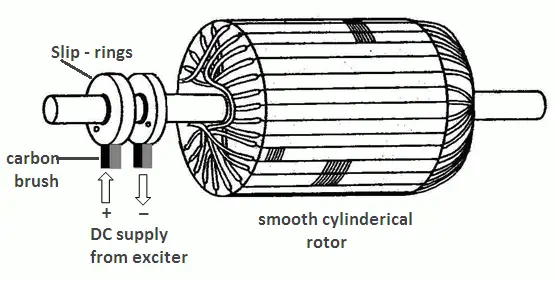
\includegraphics[width=.55\linewidth]{img/3/Synchronous-machine-rotor.png}
    \end{figure}
\end{minipage}\hfill
\begin{minipage}[c]{.5\linewidth}
    \centering
    \usetikzlibrary{shapes.arrows}
    \scalebox{0.5}{
    \begin{tikzpicture}[>=stealth,cross/.style={path picture={ 
    \draw[black]
    (path picture bounding box.south east) -- (path picture bounding box.north west) (path picture bounding box.south west) -- (path picture bounding box.north east);
    }}]
    
    
        % main circles
        \draw (0,0) circle (5cm);
        \draw (0,0) circle (3cm);
        \fill[gray!40,even odd rule] circle[radius=5cm] circle[radius=3cm];
        
        % small circles
        \foreach \X [count=\Y starting from 0] in {$a_2'$,$b_2$,$c_1'$,$a_2$,$b_1'$,$c_1$,$a_1'$,$b_1$,$c_2'$,$a_1$,$b_2$,$c_2$} { 
        \path(180-30*\Y:4) node[circle,draw, fill=white] (n\Y) {\X};
        }
        
        % Two-way arrow
        \node[blue!40,fill=blue!40,double arrow, draw, minimum height=6cm, minimum width=2.8cm, rotate=14,text=black] at (0,0) {};
        \node[blue!40,fill=blue!40,double arrow, draw, minimum height=6cm, minimum width=2.8cm, rotate=-76,text=black] at (0,0) {};
        
        % very small circles
        \foreach \X [count=\Y starting from 0] in {0,180} { 
            \draw[rotate around={\X:(0,0)}] (-1.5,0.3) circle (0.15cm);
            \draw[rotate around={\X:(0,0)}, fill=black] (-1.5,0.3) circle (0.075cm);
            \draw[rotate around={\X:(0,0)}] (-1.1,0.4) circle (0.15cm);
            \draw[rotate around={\X:(0,0)}, fill=black] (-1.1,0.4) circle (0.075cm);
            
            \draw[rotate around={\X:(0,0)}] (-0.97,1.2) circle (0.15cm);
            \draw[rotate around={\X:(0,0)},fill=black] (-0.97,1.2) circle (0.075cm);
            \draw[rotate around={\X:(0,0)}] (-0.88,0.8) circle (0.15cm);
            \draw[rotate around={\X:(0,0)},fill=black] (-0.88,0.8) circle (0.075cm);
        }
        
        \foreach \X [count=\Y starting from 0] in {-90,90} { 
            \draw[rotate around={\X:(0,0)}, cross] (-1.5,0.3) circle (0.15cm);
            \draw[rotate around={\X:(0,0)},cross] (-1.1,0.4) circle (0.15cm);
            
            \draw[rotate around={\X:(0,0)},cross] (-0.97,1.2) circle (0.15cm);
            \draw[rotate around={\X:(0,0)},cross] (-0.88,0.8) circle (0.15cm);
        }
        
        % Poles
        \node[rotate=14] at (-0.5,2) {$N$};
        \node[rotate=14] at (0.5,-2) {$N$};
        
        \node[rotate=-76] at (2,0.5) {$S$};
        \node[rotate=-76] at (-2,-0.5) {$S$};
    
    \end{tikzpicture}
    }
\end{minipage}

\vspace{1.5em}
\noindent Para esta situação já é necessário criar uma distinção entre o ângulo elétrico e o ângulo mecânico, de acordo com a distribuição espacial do campo magnético:

\begin{figure}[H]
    \centering
    \begin{tikzpicture}
        \begin{axis}[
            xlabel=\empty,
            ylabel={\( B \)},
            axis lines=center,
            ytick=\empty,
            xtick={0,1.5708,3.14159,4.71239,6.28319,7.85398,9.42478,10.99557,12.5664},
            xticklabels=\empty,
            ymin=-1, ymax=1,
            xmin=0, xmax=14,
            domain=0:4*pi,
            samples=500,
            width=12cm, height=4cm,
        ]
        
        \addplot[black, thick] {0.75*sin(deg(x))};

        \node[above, font=\small] at (13.75,0) {$\theta_m$};
        \node[below, font=\small] at (13.725,0) {$\theta$};

        \node[above, xshift=1mm,  font=\small] at (3.14159,0) {$\frac{\pi}{2}$};
        \node[below, xshift=-1mm, font=\small] at (3.14159,0) {$\pi$};

        \node[above, xshift=-1mm,  font=\small] at (6.28319,0) {$\pi$};
        \node[below, xshift=1mm, font=\small] at (6.28319,0) {$2\pi$};

        \node[above, xshift=1mm,  font=\small] at (9.42478,0) {$\frac{3\pi}{2}$};
        \node[below, xshift=-1mm, font=\small] at (9.42478,0) {$3\pi$};

        \node[above, xshift=-1mm,  font=\small] at (12.5664,0) {$2\pi$};
        \node[below, xshift=1mm, font=\small] at (12.5664,0) {$4\pi$};
        
        \end{axis}
    \end{tikzpicture}
    \caption{Distribuição espacial da indução magnética $B$ para uma máquina de 4 pólos ($\theta_m$ --- rad. mecânicos; $\theta$ --- rad. elétricos)}
    \label{fig:distrib-espacial-B}
\end{figure}

\noindent Numa máquina com $p$ pares de pólos temos $\theta = p \theta_m$ em que $\theta$ é o ângulo elétrico e $\theta_m$ o ângulo mecânico. A frequência angular da tensão induzida $\omega$ vem então:
$$
    \omega = \frac{d\theta}{dt} = p\frac{d\theta_m}{dt} = p \omega_r 
$$
em que $\omega_r$ é a velocidade ângular do rotor. E a frequência da tensão (Hz) relaciona-se com a velocidade de rotação do motor, $n_r$ (rpm), pela expressão:
$$
    f = p \frac{n_r}{60}
$$

\clearpage
\noindent A variação espacial da indução magnética $\mathbf{B}$ ao longo do entreferro é sinusoidal, i.e., $B = B_{max}\cos(p\alpha)$, em que $B_{max}$ é o valor máximo medido no centro da cabeça do pólo e $\alpha$ o ângulo que define um ponto ao longo do entreferro, medido em radianos mecânicos a partir do eixo magnético do rotor.

O fluxo magnético por pólo $\Phi$ é o integral da indução magnética ao longo de uma revolução completa
$$
    \Phi = \int_{-\pi/2}^{\pi/2} B_{max}\cos(p\alpha) \cdot lr \,d\alpha = \frac{2B_{max}lr}{p}
$$
onde $l$ é o comprimento axial do estator e $r$ o raio interior. O fluxo ligado $\Psi$ com a fase $a$ do estator (referência), admitindo um enrolamento com $N$ espiras, é dado por
$$
    \Psi = N\Phi\cos(\theta)
$$
onde $\theta$ é o ângulo do eixo do rotor em radianos elétricos, medidos a partir do eixo magnético do enrolamento da fase $a$ do estator.
$$
    \theta = p\omega_r t = \omega t
$$
$$
    \therefore \Psi = N\Phi\cos(\omega t)
$$
Pela Lei de Indução, a tensão induzida na fase $a$ é 
$$
    e = -\frac{d}{dt} \Psi = \omega N \Phi \sin(\omega t)
$$
Esta tensão induzida (\textit{força eletromotriz}), é sinusoidal, com frequência $\omega = 2\pi f$ e está desfasada $\pi/2$ em atraso relativamente ao fluxo. É costume definir o valor eficaz desta grandeza (fase-neutro):
$$
    \boxed{ E = \frac{\omega N \Phi}{\sqrt{2}} = \sqrt{2} \pi fN \Phi }
    \implies 
    e = \sqrt{2} E \sin(\omega t)
$$

%//==============================--@--==============================//%
\subsubsection{Reação do Induzido e Esquema Equivalente}

Quando o gerador está em carga e é alimentado, o sistema trifásico de correntes simétricas que se dá no enrolamento estatórico origina um campo magnético girante no entreferro, uma vez que as correntes em cada fase estão desfasadas por $120^{\circ}$ temporalmente e espacialmente. Este fenómeno designa-se por reação do induzido, i.e., a aparição deste campo magnético à velocidade de sincronismo que se soma ao campo devido à corrente de excitação.

O fluxo magnético resultante é uma combinação dos três fluxos individuais devido às correntes no estator (vamos tomar a fase $a$ como referência):
$$
    \Psi_r = L i_a + M i_b + M i_c
$$
onde $L$ e $M$ são as indutâncias própria e mutua, respetivamente. Em regime trifásico simétrico, $\sum i_x = 0$,
$$
    \therefore \Psi_r = (L - M) i_a
$$
A tensão induzida por estas correntes na fase $a$ é portanto
$$
    e_r = -\frac{d}{dt} \Psi_r = -(L - M) \frac{d i_a}{dt}
$$
A tensão aos terminais do gerador em carga é a soma da f.e.m. devido ao indutor com a tensão devido à reação do induzido
$$
    v = e + e_r = e - (L - M) \frac{d i_a}{dt}
$$
Em regime vetorial temos:
$$
    \begin{aligned}
        \mathbf{V} &= \mathbf{E} - j\omega(L - M) \mathbf{I} \\
                   &= \mathbf{E} - jX_s \mathbf{I}
    \end{aligned}
$$
Conhecendo a tensão aos terminais e a corrente, calcula-se a f.e.m. por
$$
    \mathbf{E} = \mathbf{V} + jX_s \mathbf{I}
$$
onde a grandeza $X_s$ recebe o nome de reatância síncrona. Normalmente também inclui a reatância de dispersão do estator, que não foi considerada na análise anterior. É pratica comum expressar $X_s$ em p.u., referida aos valores nominais $S_n$ e $V_n$:
$$
    X_s = X_{s_{(p.u.)}} \frac{V^2_n}{S_n}\; [\text{p.u.}]
$$

\clearpage
\noindent Em regime estacionário (trifásico simétrico) o esquema equivalente pode ser representada por

\begin{figure}[H]
    \centering
    \begin{subfigure}[b]{.475\linewidth}
        \centering
        \scalebox{0.75}{%
            \begin{circuitikz}
                %% Configure circuitikz
                \ctikzset{inductor=cute}    
                \ctikzset{inductors/coils=4}
                \ctikzset{bipoles/resistor/height=0.25}
                \ctikzset{bipoles/resistor/width=0.5}
                \ctikzset{resistors/zigs=4}
            
                \draw (0,-2) to[sV, l=$\mathbf{E}$] (0,2) 
                to[L, l=$jX_s$, -*] (4,2);
                \draw (0,-2) to[short,-*] (4,-2);

                \draw[>=stealth,->] (4,1.75) -- (4,-1.75) node[midway,right] {$\mathbf{V}$};
                \draw[>=stealth,->] (3.25,2) -- (3.35,2) node[midway,above] {$\mathbf{I}$};
            \end{circuitikz}
        }
        \caption{Esquema monofásico equivalente}
    \end{subfigure}\hfill
    \begin{subfigure}[b]{.475\linewidth}
        \centering
        \scalebox{0.925}{%
            \begin{tikzpicture}[>=latex, scale=3]
                \coordinate (E) at (0:2.5);
                \coordinate (I) at (-53.13:0.5); 
                \coordinate (I') at (-53.13:1.5);
                \coordinate (V) at (-20:1.791);
                
                % Phasors
                \draw[->,black] (0,0) -- (E) node[right, above] {$E$};
                \draw[->,black] (0,0) -- (I) node[below=0.2, left] {$I$};
                \draw[-,gray, dashed] (I) -- (I');
                \draw[->,black] (0,0) -- (V) node[left,below] {$V$};
                \draw[-,gray, dashed] (I') -- (V);
                \draw[->,black] (V) -- (E) node[below=0.25] {$j X_s I$};
            
                % Arcs
                \draw[-] (-20:0.2cm) arc (-20:-53.13:0.2cm) node[yshift=-0.2mm,xshift=2.4mm] {$\phi$};
                \draw[-] (0:0.4cm) arc (0:-20:0.4cm) node[yshift=1.5mm,xshift=2mm] {$\delta$};
            \end{tikzpicture}
        }
        \caption{Diagrama de fasores}
    \end{subfigure}
    
    \caption{Máquina síncrona como gerador}
    \label{fig:esquema-equiv-maq-sincrona}
\end{figure}

\noindent Despreza-se a resistência dos enrolamentos (valor pequeno face à reatância); admite-se que $\mathbf{I}$ está desfasado com um atraso de ângulo $\phi$ relativamente à tensão $\mathbf{V}$, e a f.e.m. $\mathbf{E}$ por um ângulo $\delta$ também relativamente à tensão, designado por ângulo de potência.

%//==============================--@--==============================//%
\subsection{Características de Funcionamento}
\subsubsection{Em Vazio e em Curto-circuito}

A característica em vazio é a curva da f.e.m. $E$ (tensão em vazio) em função da corrente de excitação $I_{exc}$, com a máquina a rodar à velocidade nominal (sincronismo), movida pela máquina de acionamento.

A curva característica em vazio exibe uma zona linear (cuja linha tangente é a reta entreferro), para valores baixos de corrente de excitação. Apresenta a não-linearidade resultante de saturação do ferro, quando o fluxo magnético excede um determinado valor limite.

Na operação próxima à tensão nominal, aproxima-se a máquina a outra fictícia que não exibe saturação, caracterizada pela reta de magnetização que passa pela origem e pelo ponto correspondente à tensão nominal.

\vspace{1em}\hrule\vspace{1em}

\noindent A característica em curto-circuito é a curva da corrente no estator $I$ em função de $I_{exc}$, com a máquina a rodar à velocidade síncrona, e os enrolamentos do estator em curto-circuito.

A curva característica em curto-circuito é linear, uma vez que o fluxo magnético tem um valor muito baixo nestas condições (não se manifesta a saturação).

\vspace{1em}\hrule\vspace{1em}

\noindent Podemos calcular a reatância $X_s$ a partir das características em vazio e em curto-circuito. Lembramos que $E \;\propto\; \omega$, ao fixarmos $I_{exc}$ correspondente à tensão nominal no ensaio em vazio, $\mathbf{E}=\mathbf{V}_n$. No ensaio em curto-circuito, $\mathbf{E}=jX_s \mathbf{I}_{cc}$, então, para o $I_{exc}$ fixo escolhido anteriormente, e como $E \;\propto\; \omega$ é um valor fixo à tensão nominal, temos que $V_n = X_s I_{cc}$, isto é:
$$
    \therefore X_s = \frac{V_n}{I_{cc}}
$$

\vspace{-1.5em}
\begin{minipage}[c]{.5\linewidth}
\begin{figure}[H]
    \centering
    \scalebox{1.15}{%
        \begin{tikzpicture}
            \begin{axis}[
                xmin=0, xmax=1,
                ymin=0, ymax=2.5,
                axis lines=middle,
                width=7cm,
                height=7cm,
                xtick=\empty, 
                ytick={1.291}, 
                yticklabels={$V_n$},
                tick style={font=\tiny},
                ytick align=outside, 
                xtick align=outside,
                ytick pos=left,
                ticklabel style = {font=\tiny},
                clip=false,
                restrict y to domain=*:2.5,
                legend pos=north west, % Position of the legend
                legend style={
                    legend columns=2,
                    font=\tiny,
                    row sep=0.05pt, % Adjust the vertical spacing between legend entries
                    column sep=1pt, % Adjust the horizontal spacing between legend image and text
                    nodes={scale=0.75, transform shape}
                },
            ]
                \node[font=\scriptsize] at (-0.04,2.5) {$E$};
                \node[font=\scriptsize] at (1.035,2.5) {$I$};
                \node[font=\scriptsize] at (1.06,-0.05) {$I_{exc}$};
        
                % OCC
                \addplot[blue!90, domain=0.1692:0.9, samples=100] ({x},{1.5*(1-1.2*exp(-5*x))});
                \addlegendentry{Em Vazio}
                
                % Entreferro
                \addplot[blue!90, domain=0:0.1692, samples=100, forget plot] ({x},{4.3*x});
                \addplot[dashed, black, domain=0:0.485, samples=100] ({x},{4.3*x});
                \addlegendentry{Entreferro}
        
                % No saturation
                \addplot[gray!50, domain=0:0.63, samples=100] ({x},{3*x});
                \addlegendentry{Reta de Magnetização}
        
                % SC
                \addplot[green!50!blue, domain=0:0.9, samples=100] ({x},{1.25*x});
                \addlegendentry{Em Curto-circuito}
        
                % relevant horizontal values
                \addplot[dotted,black, domain=0:1.291, samples=100] ({0.4302},{x});
                \addplot[dotted,black, domain=0:0.4302, samples=100] ({x},{1.291});
                \addplot[dotted,black, domain=0.4302:1, samples=100] ({x},{0.538});
            \end{axis}
            \begin{axis}[
                xmin=0, xmax=1,
                ymin=0, ymax=2.5,
                axis y line*=right,
                axis x line=none,
                axis lines=left, % Adjusted line
                ytick={0.538}, 
                yticklabels={$I_{cc}$},
                width=7cm,
                height=7cm,
                tick style={font=\tiny},
                ytick align=outside, 
                xtick align=outside,
                ytick pos=right,
                ticklabel style = {font=\tiny},
                clip=false,
                restrict y to domain=*:2.5,
            ]
            \end{axis}
        \end{tikzpicture}
    }
    \caption{Caracteristica em vazio e em curto-circuito}
    \label{fig:maq-sincrona-vazio-e-cc}
\end{figure}
\end{minipage}\hfill
\begin{minipage}[c]{.45\linewidth}
    \begin{mdframed}
        \vspace{2.25cm}
        \hfil (imagem)
        \vspace{2.25cm}
    \end{mdframed}
\end{minipage}

%//==============================--@--==============================//%
\clearpage
\subsubsection{Em Carga}

\noindent A potência nominal de uma máquina síncrona  é a máxima potência aparente à tensão nominal com fp $= 0.85,0.90, 0.95$ que pode fornecer continuamente. O fator que a limita é o aquecimento devido às correntes que percorrem os enrolamentos (limite térmico).

\begin{mdframed}
    \hfil Potência ativa $<$ potência nominal $\rightarrow$ limitada pela potência da máquina de acionamento.
\end{mdframed}

\noindent Quando a máquina está a funcionar à velocidade síncrona e está excitada de modo a apresentar a sua tensão nominal em vazio, podemos assumir que a corrente de carga aumentará gradualmente a partir de zero até atingir o seu valor nominal, mantendo um fator de potência constante.

\begin{minipage}[b]{0.5\linewidth}
   \begin{figure}[H]
        \centering
        \begin{tikzpicture}[>=latex, scale=3]
   
            \coordinate (E) at (0:2.5);
            \coordinate (I) at (-53.13:0.5); 
            \coordinate (I') at (-53.13:1.5);
            \coordinate (V) at (-20:1.791);
            
            % Phasors
            \draw[->,black] (0,0) -- (E) node[right, above] {$E$};
            \draw[->,black] (0,0) -- (I) node[below=-0.01] {$I$};
            \draw[-,gray, dashed] (I) -- (I');
            \draw[->,black] (0,0) -- (V) node[right,below] {$V$};
            \draw[-,gray, dashed] (I') -- (V);
            \draw[->,black] (V) -- (E) node[below=0.15] {$j X_s I$};
        
            % Arcs
            \draw[-] (-20:0.2cm) arc (-20:-53.13:0.2cm) node[yshift=-0.2mm,xshift=2.4mm] {$\phi$};
            \draw[-] (0:0.4cm) arc (0:-20:0.4cm) node[yshift=1.5mm,xshift=2mm] {$\delta$};
            
    \end{tikzpicture}
    \end{figure} 
\end{minipage}\hfill
\begin{minipage}[b]{0.45\linewidth}
    \noindent Do diagrama de fasores, retiramos as seguintes equações:
    $$
    \begin{aligned}
        E \sin(\delta) &= X_s I \cos(\phi)\\
        E \cos(\delta) &= V + X_s I \sin(\phi)
    \end{aligned}
    $$
    Resolvendo em ordem a $V$  e eliminando o ângulo $\delta$, obtem-se:
    
    $$
        \boxed{V = \sqrt{E^2 - X_s^2 I^2 \cos(\phi)^2} - X_s I \sin(\phi)}
    $$
\end{minipage}

\vspace{1em}
\noindent Supondo $E$ constante, \underline{a tensão $V$ vai experimentar variação}:


\hspace{-1.5em}\begin{minipage}[c]{0.45\linewidth}
\noindent Pressupondo uma máquina síncrona com reactância síncrona $X = 1$ p.u. e velocidade nominal constante, com corrente de excitação constante para a tensão nominal em vazio, observamos a variação da tensão nos terminais à medida que a corrente de carga varia de 0 a 1 p.u. para diferentes fatores de potência. \underline{Calculando os extremos}:

\vspace{0.75 em}
\noindent\textbf{Para f.p. = 1:}
$$
    \boxed{V^2 + X_s^2 I^2 = E^2}\; \rightarrow\; \text{Elipse}
$$

\noindent\textbf{Para f.p. = 0:}
$$
    \begin{aligned}
       &\text{Indutivo:}\quad &\boxed{V = E - X_s I}\\
        &\text{Capacitivo:}\quad &\boxed{V = E + X_s I}
    \end{aligned}
$$

\noindent A variação da tensão com a corrente é linear.

\end{minipage}
\begin{minipage}[c]{0.5\linewidth}
\begin{figure}[H]
    \centering
    \begin{tikzpicture}[scale=1.4]
        \begin{axis}[
            xmin=0, xmax=1,
            ymin=0, ymax=2,
            axis lines=middle,
            width=7cm,
            height=7cm,
            xtick={0,0.2,0.4,0.6,0.8,1}, 
            ytick={1}, 
            tick style={font=\tiny},
            ytick align=outside, 
            xtick align=outside,
            ytick pos=left,
            ticklabel style = {font=\tiny},
            clip=false
        ]
    
            \node[font=\scriptsize] at (-0.06,1.95) {$V_\text{p.u.}$};
            \node[font=\scriptsize] at (1.06,-0.05) {$I_\text{p.u.}$};
            
             % Plot for delta = 0 ind and cap
            \addplot[black, domain=0:1, samples=100] {1 - x} node[right, font=\tiny] at (axis cs:0.7,0.15) {0 ind};
            \addplot[black, domain=0:1, samples=100] {1 + x} node[right, font=\tiny] at (axis cs:0.7,1.85) {0 cap};
            
            % Plot for delta = 0.85 ind and cap
            \addplot[black,dashed, domain=0:1, samples=100] {sqrt(1 - 0.85^2*x^2) - x*0.52678} node[right, font=\tiny] at (axis cs:0.7,0.43) {0.85 ind};
            \addplot[black,dashed, domain=0:1, samples=100] {sqrt(1 - 0.85^2*x^2) + x*0.52678} node[right, font=\tiny] at (axis cs:0.7,1.2) {0.85 cap};
            
            % Plot for delta = 1
            \addplot[black,densely dotted, domain=0:1, samples=100] {sqrt(1 - x^2)} node[right, font=\tiny] at (axis cs:0.7,0.73) {1};
        \end{axis}
    \end{tikzpicture}
\end{figure} 
\end{minipage}

\vspace{0.5em}
\begin{mdframed}
    \begin{enumerate}
        \item Quando o fator de potência é unitário ou indutivo:
        \begin{itemize}
            \item A tensão diminui à medida que a corrente de carga aumenta.
            \item Isso ocorre devido ao efeito desmagnetizante da reação do induzido, onde o fluxo magnético se subtrai do fluxo principal.
        \end{itemize}
    
        \item Quando o fator de potência é capacitivo:
        \begin{itemize}
            \item A tensão aumenta à medida que a corrente de carga.
            \item Isso ocorre porque a reação do induzido tem um efeito magnetizante, onde o fluxo magnético se soma ao fluxo principal, especialmente em correntes relativamente baixas.
        \end{itemize}
    \end{enumerate}
\end{mdframed}

\clearpage
\noindent Se se pretender  manter constante a tensão então há que \underline{atuar sobre a corrente de excitação que condiciona $E$}. Para uma dada potência ativa, sendo a amplitude de tensão $V$ constante a variação da corrente de excitação altera $E$ donde resulta uma variação de intensidade $I$ e $\sin(\phi)$. A equação anterior pode reescrever-se:

$$
    \boxed{E = \sqrt{V^2 + X_s^2I^2 + 2V X_s I \sin(\phi)}}
$$

\hspace{-1.5em}\begin{minipage}[c]{0.45\linewidth}
\noindent Pressupondo novamente a máquina síncrona com reactância síncrona $X = 1$ p.u. com tensão nominal aos terminais, observamos a variação da f.e.m $E$ à medida que a corrente de carga varia de 0 a 1.0 p.u. para diferentes fatores de potência e potência ativa. \underline{Calculando os extremos}:

\vspace{1 em}
\noindent\textbf{Para P = 0:}
$$
    \boxed{E = V \pm X_s I}\; \rightarrow\; \text{Linear}
$$
$\cos(\phi) = 0$ e consequentemente, $\sin(\phi) = \pm 1$
\noindent\textbf{Para P = 1:}

$$
    \begin{aligned}
            &E = \sqrt{V^2 + X_s^2 I^2}\\
            &\boxed{E^2 - I^2 = 1}\; \rightarrow\; \text{Hiperbole}
    \end{aligned}
$$
$\cos(\phi) = 1$ e consequentemente, $\sin(\phi) = 0$

\vspace{0.5em}
\noindent O fator de potência encontra-se representado a traço interrompido.

\end{minipage}
\begin{minipage}[c]{0.5\linewidth}
\begin{figure}[H]
    \centering
\begin{tikzpicture}[scale=1.4]
    \begin{axis}[
        xmin=0, xmax=1.1,
        ymin=0, ymax=2,
        axis lines=middle,
        width=7cm,
        height=7cm,
        xtick={0,0.2,0.4,0.6,0.8,1}, 
        ytick={1}, 
        tick style={font=\tiny},
        ytick align=outside, 
        xtick align=outside,
        ytick pos=left,
        ticklabel style = {font=\tiny},
        clip=false,
        restrict x to domain=*:1,
    ]

        \node[font=\scriptsize] at (-0.07,1.95) {$E_\text{p.u.}$};
        \node[font=\scriptsize] at (1.16,-0.05) {$I_\text{p.u.}$};

        % Plot for FP = 1
        \addplot [gray,dashed,domain=0:1, samples=100] {sqrt(x^2 + 1)};

        % Plot for FP = 0.85 cap
        \addplot [gray,dashed,domain=0:1, samples=100] {sqrt(x^2 + 2*0.5267*x + 1)};

        % Plot for FP = 0.85 ind
        \addplot [gray,dashed,domain=0:1, samples=100] {sqrt(x^2 - 2*0.5267*x + 1)};
        
         % Plot for P = 0
        \addplot[black, domain=0:1, samples=100] {1 - x};
        \addplot[black, domain=0:1, samples=100] {1 + x};

         % Plot for P = 1
        \addplot [black, samples=200] ({sqrt(x^2 + 1)-0.05},{x+1.45});

        % Plot for P = 0.5
        \addplot [black, samples=200] ({sqrt(x^2 + sqrt(3)*x + 1)},{x + 2});

        % Plot for P = 0.25
       \addplot [black, samples=200] ({sqrt(x^2 + 0.9682*2*x + 1)},{x + 2});

        % Plot for P = 0.75
        \addplot [black, samples=200] ({sqrt(x^2 + 2*0.6613*x + 1)},{x + 2});


        % Lengends
        \node[font=\tiny] at (1.0195,0.03) {$0$};
        \node[font=\tiny] at (1.05,0.15) {$0.25$};
        \node[font=\tiny] at (1.035,0.35) {$0.5$};
        \node[font=\tiny] at (1.05,0.75) {$0.75$};
        \node[font=\tiny] at (1.0195,1.2) {$1$};

        \node[gray, font=\tiny] at (1.1,1) {$0.85$ cap};
        \node[gray, font=\tiny] at (1.1,1.8) {$0.85$ ind};
        \node[gray, font=\tiny] at (1.0195,1.45) {$1$};

    \end{axis}
\end{tikzpicture}
\end{figure} 
\end{minipage}

\vspace{0.5em}
\begin{mdframed}
    \begin{enumerate}
        \item  O valor da corrente te carga é mínimo para f.p $= 1$ (O traço interrompido interceta as curvas hiperbólicas no mínimo relativo ao eixo das abcissas) aumentando à medida que o fator de potência diminui.

        \item Quando traçadas em função da corrente de excitação, estas curvas são conhecidas pela designação de curvas em V. O seu andamento é semelhante ao gráfico da variação da tensão, ainda que não idêntico, por força da saturação da característica em vazio $E(I_\text{exc})$.
    \end{enumerate}
\end{mdframed}

%//==============================--@--==============================//%
\subsubsection{Fórmulas da Potência Ativa e Reativa}

\noindent Tomando a tensão aos terminais de V como referência, a potência complexa fornecida pelo gerador é:

$$
\begin{aligned}
      \mathbf{S}_G = P_G + jQ_G = &\mathbf{V}\mathbf{I}^* = V e^{j 0} e^{j \phi} = VI e^{j \phi}\\
      P_G = V I \cos(\phi)&\qquad
      Q_G = V I \sin(\phi)
\end{aligned}
$$

\noindent Relembrando as expressões do diagrama de fasores, podemos escrever as potências ativa e reativa da seguinte forma:
$$
    \left\{\begin{aligned}
        E \sin(\delta) &= X_s I \cos(\phi)\\
        E \cos(\delta) &= V + X_s I \sin(\phi)
    \end{aligned}\right.\quad
    \rightarrow\quad
    \left\{\begin{aligned}
         P_G &= \frac{E V}{X_s} \sin(\delta)\\
         Q_G &= \frac{V}{X_s} \left(E\cos(\delta) - V\right) =  \frac{V}{X_s} \Delta
    \end{aligned}\right.\qquad
$$

\noindent O ângulo de potência $\delta$ não é uma variável de controlo. Sendo o gerador um conversor mecanoeléctrico, a potência ativa gerada é (à parte as perdas) igual à potência mecânica fornecida pela máquina motriz. Note-se que $\delta$ depende da f.e.m. $E$ e, por conseguinte, da corrente de excitação:

\begin{mdframed}
    \noindent Constata-se que a potência reativa depende da diferença $\Delta$. Admitindo constante a tensão V:
    $$
        \begin{aligned}
            &E \cos(\delta) = V\; \rightarrow\; \text{A potência reativa é controlável através da corrente de excitação que determina a $E$.}\\
            &\mkern140mu \text{A excitação normal é definida para $\delta$ = 0.}\\
            &E \cos(\delta) > V\; \rightarrow\; \text{A máquina fica sobreexcitada e fornece potência reativa.}\\
            &E \cos(\delta) < V\; \rightarrow\; \text{A máquina fica subexcitada e absorve potência reativa.}
        \end{aligned}
    $$
\end{mdframed}

%//==============================--@--==============================//%

    \clearpage
    \section{Linha Elétrica de Energia}%
        \setcounter{figure}{29}

%//==============================--@--==============================//%

A transmissão de energia elétrica é realizada pelo campo eletromagnético criado pela tensão entre os condutores e pela corrente que neles flui.

As linhas são normalmente aéreas, constituidas por condutores de alumímio ou de cobre. Os condutores (sujeitos ao peso e uma força longitudinal) descrevem uma linha designada por \textit{catenária}, a qual para pequenas distancias se aproximada de uma parábola.

A tensão nominal de uma linha determina a sua capacidade de transporte, i.e., quanto maior a tensão, maior é a potência transmitida. As tensões mais elevadas requerem naturalmente um isolamento mais pronunciado, bem como maiores distâncias entre condutores e entre estes e a terra. 

%//==============================--@--==============================//%
\subsection{Modelos da Linha em Regime Estacionário}

\subsubsection{Modelo Exato}

Considerando um troço de uma fase de uma linha com comprimento infinitesimal $dx$, onde $v$ é a tensão fase-neutro e $i$ a corrente por fase, funções do tempo e da distância $x$ medida a partir do emissor, podemos escrever:
$$
    \left\{
    \begin{aligned}
        v(x) - v(x+dx) &= R\, dx\, i + L\, dx\, \frac{\partial i}{\partial t} \\[8pt]
        i(x) - i(x+dx) &= G\, dx\, v + C\, dx\, \frac{\partial v}{\partial t}
    \end{aligned}\right.
    \quad\implies\quad
    \left\{
    \begin{aligned}
        -\frac{\partial v}{\partial x} &= Ri + L\frac{\partial i}{\partial t} \\[8pt]
        -\frac{\partial i}{\partial x} &= Gv + C\frac{\partial v}{\partial t}
    \end{aligned}\right.
    \quad\implies\quad
    \left\{
    \begin{aligned}
        -\frac{\partial \mathbf{V}}{\partial x} &= (R + j\omega L) \mathbf{I} \\[8pt]
        -\frac{\partial \mathbf{I}}{\partial x} &= (G + j\omega C) \mathbf{V}
    \end{aligned}\right.
$$

% \vspace{-1em}
% \begin{figure}[H]
%     \centering
%     \scalebox{1.0}{%
%         \begin{circuitikz}
%             %% Esquema equivalente em pi
%             \draw (0,0) 
%                 to[short, *-] (2,0)
%                 to[generic, l=$\mathbf{B}$] (7,0)
%                 to[short, -*] (9,0);

%             \draw (2,0) to[generic, l=$\displaystyle \frac{\mathbf{A}-1}{\mathbf{B}}$] (2,-3);
%             \draw (7,0) to[generic, l_=$\displaystyle \frac{\mathbf{A}-1}{\mathbf{B}}$] (7,-3);

%             \draw (0,-3) to[short, *-*] (9,-3);

%             %% Labels e arrows
%             \draw[>=stealth,->] (0,-0.25) -- (0,-2.75) node[midway,left] {$\mathbf{V}_e$};
%             \draw[>=stealth,->] (9,-0.25) -- (9,-2.75) node[midway,right] {$\mathbf{V}_r$};
%         \end{circuitikz}
%     }
%     \caption{Esquema equivalente monofásico de uma linha com parâmetros distribuidos}
%     \label{fig:linha-esq-monofasico}
% \end{figure}

\noindent Definem-se a característica (ou impedância) da onda $\mathbf{Z}_0$ ($\Omega$) e constante de propagação $\gamma$ (m$^{-1}$):
$$
    \begin{aligned}
        \mathbf{Z}_0 &= \sqrt{\frac{R + j\omega L}{G + j\omega C}} = \sqrt{\frac{R + jX}{G + jB}} \\
        \gamma &= \sqrt{(R + j\omega L)(G + j\omega C)} = \sqrt{(R + jX)(G + jB)} = \alpha + j\beta
    \end{aligned}
$$
onde $\alpha$ é o fator de atenuação e $\beta$ o fator de desfasagem. 

Para obtermos as soluções definimos as seguintes EDOs, após derivar e substituir:
$$
    \left\{
    \begin{aligned}
        \frac{d^2 \mathbf{V}}{dx^2} &= (R + j\omega L)(G + j\omega C) \mathbf{V} \\[6pt]
        \frac{d^2 \mathbf{I}}{dx^2} &= (R + j\omega L)(G + j\omega C) \mathbf{I}
    \end{aligned}\right.
    \quad\iff\quad
    \left\{
    \begin{aligned}
        \frac{d^2 \mathbf{V}}{dx^2} &= \gamma^2\, \mathbf{V} \\[6pt]
        \frac{d^2 \mathbf{I}}{dx^2} &= \gamma^2\, \mathbf{I}
    \end{aligned}\right.
    \quad\implies\quad
    \boxed{%
    \begin{aligned}
        \mathbf{V} &= \mathbf{V}_e \cosh(\gamma x) - \mathbf{Z}_0 \mathbf{I}_e \sinh(\gamma x) \\[4pt]
        \mathbf{I} &= -\frac{\mathbf{V}_e}{\mathbf{Z}_0} \sinh(\gamma x) + \mathbf{I}_e \cosh{\gamma x}
    \end{aligned}}
$$
As soluções obtidas são para uma distância qualquer entre o emissor e o recetor. Interessa o caso específico no extremo do recetor ($\mathbf{V}_r, \mathbf{I}_r$) em que $x = d$. Sob a forma matricial temos:
$$
    \begin{bmatrix}
        \mathbf{V}_r \\[6pt]
        \mathbf{I}_r
    \end{bmatrix}
    =
    \begin{bmatrix}
        \cosh(\gamma d) & -\mathbf{Z}_0 \sinh(\gamma d) \\[6pt]
        -1/\mathbf{Z}_0 \cdot \sinh(\gamma d) & \cosh(\gamma d)
    \end{bmatrix}
    \begin{bmatrix}
        \mathbf{V}_e \\[6pt]
        \mathbf{I}_e
    \end{bmatrix}
    \iff 
    \begin{bmatrix}
        \mathbf{V}_e \\[6pt]
        \mathbf{I}_e
    \end{bmatrix}
    =
    \begin{bmatrix}
        \cosh(\gamma d) & \mathbf{Z}_0 \sinh(\gamma d) \\[6pt]
        1/\mathbf{Z}_0 \cdot \sinh(\gamma d) & \cosh(\gamma d)
    \end{bmatrix}
    \begin{bmatrix}
        \mathbf{V}_r \\[6pt]
        \mathbf{I}_r
    \end{bmatrix}
$$
Podemos apresentar a equação sob a forma:
$$
    \begin{bmatrix}
        \mathbf{V}_e \\[6pt]
        \mathbf{I}_e
    \end{bmatrix}
    =
    \begin{bmatrix}
        \mathbf{A} & \mathbf{B} \\[6pt]
        \mathbf{C} & \mathbf{D}
    \end{bmatrix}
    \begin{bmatrix}
        \mathbf{V}_r \\[6pt]
        \mathbf{I}_r
    \end{bmatrix}
$$
em que os parâmetros $\mathbf{A}$, $\mathbf{B}$, $\mathbf{C}$ e $\mathbf{D}$ são dados por:
$$
    \begin{aligned}
        \mathbf{A} &= \mathbf{D} = \cosh(\gamma d) = \cosh(\sqrt{\mathbf{Z}_L \mathbf{Y}_T}) \\[1pt]
        \mathbf{B} &= \mathbf{Z}_0 \sinh(\gamma d) = \frac{\mathbf{Z}_0 \sinh(\sqrt{\mathbf{Z}_L \mathbf{Y}_T})}{\sqrt{\mathbf{Z}_L \mathbf{Y}_T}} \\[1pt]
        \mathbf{C} &= \frac{\sinh(\gamma d)}{\mathbf{Z}_0} = \frac{\mathbf{Y}_T \sinh(\sqrt{\mathbf{Z}_L \mathbf{Y}_T})}{\sqrt{\mathbf{Z}_L \mathbf{Y}_T}}
    \end{aligned}
$$
onde $\mathbf{Z}_L = (R + j\omega L)d$ e $\mathbf{Y}_T = (G + j\omega C)d$ são a impedância longitudinal e admitância transversal totais, respetivamente.

\begin{mdframed}
    Para uma \underline{linha sem perdas}, a impedância longitudinal e a admitância transversal são imaginários puros, logo, a impedância característica e a constante de propagação são real e imaginária pura, respetivamente:
    $$
        \mathbf{Z_0} = \sqrt{\dfrac{L}{C}}
        \qquad\quad
        \gamma = j\omega\sqrt{LC} = j\beta, \quad \text{onde $\beta$ é a constante de fase}
    $$
\end{mdframed}

%//==============================--@--==============================//%
\subsubsection{Esquema em $\pmb{\pi}$ Exato}

Para a modelação da linha numa rede interligada é conveniente utilizarmos um esquema equivalente em $\pi$ como se apresenta \hyperref[fig:linha-transmissao-esq-exato]{em baixo}. O ramo longitudinal possui uma impedância $\mathbf{B}$ e os dois ramos transversais uma admitância $(\mathbf{A}-1)/\mathbf{B}$.

\vspace{-1.25em}
\begin{figure}[H]
    \centering
    \scalebox{1.0}{%
        \begin{circuitikz}
            %% Esquema equivalente em pi
            \draw (0,0) 
                to[short, *-] (2,0)
                to[generic, l=$\mathbf{B}$] (7,0)
                to[short, -*] (9,0);

            \draw (2,0) to[generic, l=$\displaystyle \frac{\mathbf{A}-1}{\mathbf{B}}$] (2,-3);
            \draw (7,0) to[generic, l_=$\displaystyle \frac{\mathbf{A}-1}{\mathbf{B}}$] (7,-3);

            \draw (0,-3) to[short, *-*] (9,-3);

            %% Labels e arrows
            \draw[>=stealth,->] (0,-0.25) -- (0,-2.75) node[midway,left] {$\mathbf{V}_e$};
            \draw[>=stealth,->] (9,-0.25) -- (9,-2.75) node[midway,right] {$\mathbf{V}_r$};
        \end{circuitikz}
    }
    \caption{Esquema equivalente em $\pi$ exato}
    \label{fig:linha-transmissao-esq-exato}
\end{figure}

%//==============================--@--==============================//%
\subsubsection{Esquema em $\pmb{\pi}$ Nominal (linhas médias)}

Os valores da impedância longitudinal e admitâncias transversais no esquema em $\pi$ são, respetivamente:
$$
    \begin{aligned}
        \mathbf{B} &= \mathbf{Z}_0 \sinh(\gamma d) \\[1pt]
        \frac{\mathbf{A}-1}{\mathbf{B}} &= \frac{\cosh(\gamma d)-1}{\mathbf{Z}_0 \sinh(\gamma d)} = \frac{1}{\mathbf{Z}_0} \tanh\left(\frac{\gamma d}{2}\right)
    \end{aligned}
$$
Para linhas em que $d \le 250\;$km, verifica-se que $\gamma d \ll 1$, o que implica que $\sinh(\gamma d) \approx \gamma d$ e $\tanh(\gamma d/2) \approx \gamma d/2$.

Esta simplificação resulta em:
$$
    \begin{aligned}
        \mathbf{B} &= \mathbf{Z}_0\, \gamma d = \sqrt{\frac{\mathbf{Z}_L}{\mathbf{Y}_T}}\, \sqrt{\mathbf{Z}_L \mathbf{Y}_T} = \mathbf{Z}_L \\[1pt]
        \frac{\mathbf{A}-1}{\mathbf{B}} &= \frac{1}{\mathbf{Z}_0} \frac{\gamma d}{2} = \sqrt{\frac{\mathbf{Y}_T}{\mathbf{Z}_L}}\, \frac{\sqrt{\mathbf{Z}_L \mathbf{Y}_T}}{2} = \frac{\mathbf{Y}_T}{2}
    \end{aligned}% Hallo :3 minminnho
$$
o que se traduz na simplificação do esquema equivalente apresentado na \hyperref[fig:linha-transmissao-esq-nominal]{Fig. 31}.

\vspace{-0.5em}
\begin{figure}[H]
    \centering
    \scalebox{1.0}{%
        \begin{circuitikz}
            %% Esquema equivalente em pi
            \draw (0,0) 
                to[short, *-] (2,0)
                to[generic, l=$\mathbf{Z}_L$] (7,0)
                to[short, -*] (9,0);

            \draw (2,0) to[generic, l=$\displaystyle \frac{\mathbf{Y}_T}{2}$] (2,-3);
            \draw (7,0) to[generic, l_=$\displaystyle \frac{\mathbf{Y}_T}{2}$] (7,-3);

            \draw (0,-3) to[short, *-*] (9,-3);

            %% Labels e arrows
            \draw[>=stealth,->] (0,-0.25) -- (0,-2.75) node[midway,left] {$\mathbf{V}_e$};
            \draw[>=stealth,->] (9,-0.25) -- (9,-2.75) node[midway,right] {$\mathbf{V}_r$};
        \end{circuitikz}
    }
    \caption{Esquema equivalente em $\pi$ nominal}
    \label{fig:linha-transmissao-esq-nominal}
\end{figure}

\vspace{-0.5em}
\noindent As equações do esquema em $\pi$ nominal escrevem-se:
$$
    \begin{bmatrix}
        \mathbf{V}_r \\[10pt]
        \mathbf{I}_r
    \end{bmatrix}
    =
    \begin{bmatrix}
        1+\dfrac{\mathbf{Z}_L\mathbf{Y}_T}{2} & -\mathbf{Z}_L \\[10pt]
        -\mathbf{Y}_T \left(1+\dfrac{\mathbf{Z}_L\mathbf{Y}_T}{4}\right) & 1+ \dfrac{\mathbf{Z}_L\mathbf{Y}_T}{2}
    \end{bmatrix}
    \begin{bmatrix}
        \mathbf{V}_e \\[10pt]
        \mathbf{I}_e
    \end{bmatrix}
    \iff
    \begin{bmatrix}
        \mathbf{V}_e \\[10pt]
        \mathbf{I}_e
    \end{bmatrix}
    =
    \begin{bmatrix}
        1+\dfrac{\mathbf{Z}_L\mathbf{Y}_T}{2} & \mathbf{Z}_L \\[10pt]
        \mathbf{Y}_T \left(1+\dfrac{\mathbf{Z}_L\mathbf{Y}_T}{4}\right) & 1+ \dfrac{\mathbf{Z}_L\mathbf{Y}_T}{2}
    \end{bmatrix}
    \begin{bmatrix}
        \mathbf{V}_r \\[10pt]
        \mathbf{I}_r
    \end{bmatrix}
$$
%//==============================--@--==============================//%
\subsubsection{Nota sobre Funções Hiperbólicas}

As funções hiperbólicas têm uma relação intima com as funções trigonométricas, como revelam as definições:

\vfill
\begin{center}
    \setlength{\tabcolsep}{0.75cm}
    \begin{tabular}{c|c|c}
         $\cosh(u) = \dfrac{e^{u} + e^{-u}}{2}$ & $\sinh(v) = \dfrac{e^{v}-e^{-v}}{2}$ & $\tanh(w) = \dfrac{\sinh(w)}{\cosh(w)} = \dfrac{e^{w}-e^{-w}}{e^{w} + e^{-w}}$ \\[12pt]
         $\cos(u) = \dfrac{e^{ju} + e^{-ju}}{2}$ & $\sin(v) = \dfrac{e^{jv}-e^{-jv}}{2j}$ & $\tan(w) = \dfrac{\sin(w)}{\cos(w)} = \dfrac{e^{jw}-e^{-jw}}{j(e^{jw} + e^{-jw})}$ \\
         & & \\
         \bottomrule
         & & \\
         $\therefore \cos(u) = \cosh(ju)$ & $\therefore j\sin(v) = \sinh(jv)$ & $\therefore j\tan(w) = \tanh(jw)$
    \end{tabular}  
\end{center}

%//==============================--@--==============================//%
\clearpage
\subsection{Linha Terminada pela Impedância de Onda}

%//==============================--@--==============================//%
\subsubsection{Linha com Perdas}

Se a linha for terminada por $\mathbf{Z}_0$, a relação entre a tensão e a corrente ao longo da linha simplifica-se consideravelmente. Temos, neste caso, $\mathbf{V}_r = \mathbf{Z}_0\, \mathbf{I}_r$, o que leva à reconstrução da relação:
$$
    \begin{aligned}
        \mathbf{V}_e &= (\cosh(\gamma d) + \sinh(\gamma d))\, \mathbf{V}_r = e^{\gamma d}\, \mathbf{V}_r\\
        \mathbf{I}_e &= (\sinh(\gamma d) + \cosh(\gamma d))\, \mathbf{I}_r = e^{\gamma d}\, \mathbf{I}_r
    \end{aligned}
$$
Dividindo as expressões anteriores, descobrimos a relação:
$$
    \frac{\mathbf{V}_e}{\mathbf{I}_e} = \frac{\mathbf{V}_r}{\mathbf{I}_r} = \mathbf{Z}_0
$$
Este resultado implica que na emissão a linha apresenta, tal como na receção, a impedância de onda. Verifica-se esta relação para qualquer outro ponto genérico da mesma.

% \vspace{}
\noindent\begin{minipage}[c]{0.45\linewidth}
    \begin{figure}[H]
        \centering
        \scalebox{0.65}{%
            \begin{tikzpicture}[>=stealth]
                \coordinate (O) at (0,0);
        
                \draw[thick,->] (O) -- (350:5cm) node[above=3mm,left] {$\mathbf{V}_e$};
                \draw[thick,->] (O) -- (10:2.6cm) node[above,left=1.5mm,yshift=2mm] {$\mathbf{I}_e$};
                \draw[dashed] (O) circle(5cm);
        
                \draw[thick,->] (O) -- (290:5cm) node[above=3mm,right,xshift=-0.5mm,yshift=2mm] {$\mathbf{V}_r$};
                \draw[thick,->] (O) -- (310:2.6cm) node[above,right=1.5mm,xshift=-0.75mm,yshift=-0.75mm] {$\mathbf{I}_r$};
                \draw[dashed] (O) circle(2.6cm);
    
                \draw[<->,thin] (290:1.5cm) arc (290:350:1.5cm)
                node[midway,above,xshift=4mm,yshift=-2mm] {$\beta d$};
            \end{tikzpicture}
        }
        \caption{Tensão e corrente numa linha terminada por $\mathbf{Z}_0$}
    \end{figure}
\end{minipage}\hfill
\begin{minipage}[c]{0.5\linewidth}
    A constante de propagação é um número complexo, i.e., $\gamma = \alpha + j\beta$. Substituindo, vem que
    $$
        \frac{V_r}{V_e} = \frac{I_r}{I_e} = e^{-\alpha d}
    $$
    $$
        \arg(\mathbf{V}_e)-\arg(\mathbf{V}_r) = \arg(\mathbf{I}_e) - \arg(\mathbf{I}_r) = \beta d
    $$
    Conclui-se que a tensão e a corrente ao longo da linha se vão atenuando da emissão para a receção com o fator de atenuação $\alpha$, ao mesmo tempo que sofrem uma rotação no sentido negativo, com o fator de desfasagem $\beta$. A impedância de onda é tipicamente capacitiva (argumento entre $0^{\circ}$ e $-15^{\circ}$), pelo que a corrente está avançada em relação à tensão. A atenuação e a rotação variam linearmente com o comprimento da linha (na representação ao lado a atenuação não é muito acentuada).
\end{minipage}


%//==============================--@--==============================//%
\subsubsection{Linha sem Perdas}

Como já mencionado acima, admitindo uma linha sem perdas, temos uma impedância de onda resistiva pura e uma constante de propagação imaginária pura (sem nulo o fator de atenuação):
$$
    \mathbf{Z_0} = \sqrt{\dfrac{L}{C}}
    \qquad\quad
    \gamma = j\omega\sqrt{LC} = j\beta,\; \text{ em que $\beta = \omega \sqrt{LC}$}
$$
A velocidade da onda eletromagnética ao longo da linha pode ser dada por $\nu = 1/\sqrt{LC}$, de que resulta:
$$
    \beta = \frac{\omega}{\nu}
$$
O comprimento de onda $\lambda$ é dado por pela relação:
$$
    \lambda = \frac{\nu}{f} = 2\pi \frac{\nu}{\omega}
$$
A desfasagem entre as tensões na emissão e na receção podem então escrever-se como:
$$
    \beta d = 2\pi \frac{d}{\lambda}
$$

\vspace{0.25em}\hrule\vspace{0.5em}

\noindent Uma vez que $\alpha = 0$, as amplitude da tensão e da corrente ao longo da linha (que estão em fase) mantêm-se constantes, o que resulta em:
$$
    \frac{V}{I} = Z_0
$$
Supondo que trabalhamos à tensão nominal, a linha transporta a \textit{potência natural} $P_n$:
$$
    P_n = \frac{V^2_n}{Z_0}
$$
Nestas condições, $\omega C d V^2 = \omega L d I^2$, i.e., ``\textit{a potência reativa gerada pela capacitância da linha iguala a absorvida pela respetiva reatância}''\cite{paiva2005}. Caso a carga seja superior a $Z_0$, a linha gera potência reativa e a tensão sobe ao longo da linha, $V_r > V_e$. O reciproco ocorre para cargas inferiores a $Z_0$ (a linha consome reativa, e $V_r < V_e$).
%//==============================--@--==============================//%
\newpage
\subsection{Capacidade de Transporte}

\subsubsection{Limite Térmico}

 Uma linha elétrica tem a sua capacidade de transporte influenciada pelo aumento da temperatura. Este aumento é causado pelas perdas devido ao efeito de Joule, que ocorrem com a passagem da corrente elétrica. A temperatura sobe até que a taxa de dissipação de calor equilibre a potência de perdas, tendo o seu valor máximo de ser limitado.
 
\begin{itemize}
    \item O \textbf{limite térmico} determina a capacidade de transporte em cabos subterrâneos e linhas de curta ou média distância (inferior a 150-200 km).
    
    \item Os cabos subterrâneos são isolados e o seu isolamento pode ser danificado se a temperatura ultrapassar um valor máximo entre 90 e 120°C.
    
    \item Os condutores das linhas aéreas expandem-se com o aumento da temperatura. Tal altera a sua trajetória (a catenária dilata), reduzindo a distância a objetos próximos. 
    
    \item O limite térmico destas linhas varia com a temperatura exterior. Por exemplo, a 35°C, é aproximadamente $2/3$ do valor a 15°C. Devido a esta característica, a capacidade de transporte no verão é notavelmente menor do que no inverno.
\end{itemize}

\subsubsection{Limite de Estabilidade Estática}

\noindent Num sistema com dois barramentos, ambos com geração e carga, ligados por uma linha com geradores que mantêm estáveis as amplitudes das tensões nos barramentos, ignorando a admitância transversal da linha, a corrente no sentido de $1 \rightarrow 2$ e a potência complexa na emissão são:

\vspace{-0.25em}
\hspace{-1.5em}\begin{minipage}[c]{0.5\linewidth}
    \begin{figure}[H]
        \centering
        \begin{circuitikz}[scale=1.2]
            \draw (7.5,12.7) to[sinusoidal voltage source, sources/symbol/rotate=auto] (7.5,12);
            \draw [thick, -](6.5,11.5) to[short] (8.5,11.5);
            \draw [thick, >=stealth,->](7.5,12) to[short] (7.5,11.5);
            \draw [>=stealth,->](7,11.5) to[short] (7,10);
             \node[yshift=-1mm,xshift=2mm,font=\normalsize] at (6.1,11.6) {$\mathbf{V}_1$};
            
            \draw (11,12.7) to[sinusoidal voltage source, sources/symbol/rotate=auto ] (11,12);
            \draw [thick, -](10,11.5) to[short] (12,11.5);
            \draw [thick, >=stealth,->](11,12) to[short] (11,11.5);
            \draw [>=stealth,->](11.5,11.5) to[short] (11.5,10);
             \node[yshift=-1mm,xshift=2mm,font=\normalsize] at (12,11.6) {$\mathbf{V}_2$};
            
            \draw [-](8,11.5) to[short] (8,11);
            \draw [-](8,11) to[short] (10.5,11);
            \draw [>=stealth,->](9.25,11) to[short] (9.3,11) node[below, font=\normalsize] {$\mathbf{I}$};
            \draw [-](10.5,11.5) to[short] (10.5,11);
        \end{circuitikz}
    \end{figure} 
\end{minipage}
\begin{minipage}[c]{0.45\linewidth}
    $$
    \mathbf{I} = \dfrac{\mathbf{V_1} - \mathbf{V_2}}{R_L + j X_L}\qquad
    \mathbf{S_{12}} = \mathbf{V_1 I^*} = \dfrac{V_1^2 - V_1 V_2 e^{j \theta}}{R_L - j X_L}
    $$

    \vspace{1em}
    onde $R_L$ e $X_L$ são a resistência e a reatância da linha e $\theta$ a desfasagem entre $V_1$ e $V_2$.
\end{minipage}

\vspace{0.75em}
\noindent A partes reais e imaginária da potência complexa fornecem a potência ativa e reativa:

$$
    \begin{aligned}
        P_{12} &= V_1^2\dfrac{R_L}{R^2_L + X^2_L} + V_1V_2\dfrac{X_L\sin(\theta) - R_L \cos(\theta)}{R^2_L + X^2_L}\\
        Q_{12} &= V_1^2\dfrac{X_L}{R^2_L + X^2_L} + V_1V_2\dfrac{X_L\cos(\theta)+ R_L \sin(\theta)}{R^2_L + X^2_L}\\   
    \end{aligned}
$$

\noindent Considerando que a potência ativa transmitida pela linha, convencionalmente positiva no sentido $1 \rightarrow 2$, é o valor médio das potência na emissão e na receção (parte real da potência complexa negada):
$$
    P = \dfrac{P_{12} - P_{21}}{2} = \dfrac{R_L}{R^2_L + X^2_L}\frac{V_1^2 - V_2^2}{2} + \frac{X_L}{R^2_L + X^2_L}V_1 V_2 \sin(\theta)
$$
\noindent Admitindo que $V_1 = V_2 = V_n$:
$$
    P = \frac{X_L}{R^2_L + X^2_L}V_n^2 \sin(\theta) = P_\text{máx}\sin(\theta)\;\rightarrow\; \boxed{P_\text{máx} = \frac{X_L}{R^2_L + X^2_L}V_n^2 \simeq \frac{V_n^2}{X_L}}
$$

\begin{mdframed}
    \begin{enumerate}
        \item A capacidade de transporte da linha aumenta quadraticamente com a tensão.
        \item A capacidade de transporte é inversamente proporcional à reatância da linha.
        \item O valor máximo do trânsito de potência ativa ocorre para $\theta = \pm \pi/2$, que corresponde ao \underline{limite de estabilidade estática} da marcha síncrona dos dois geradores:
        $$
            C_s = \dfrac{\partial P}{\partial \theta} = P_\text{máx}\cos(\theta)
        $$
        Quando $\theta = \pm \pi/2$, o coeficiente anula-se, perdendo o sincronismo entre geradores.
    \end{enumerate}
\end{mdframed}

%//==============================--@--==============================//%
\subsubsection{Limite de Estabilidade da Tensão}
\noindent Considere-se um sistema com dois barramentos ligados por uma linha, no qual um gerador ligado a um barramento alimenta uma carga ligado ao outro:

\begin{figure}[H]
    \centering
    \begin{circuitikz}[scale=1.2]
        \draw (7.5,12.7) to[sinusoidal voltage source, sources/symbol/rotate=auto] (7.5,12);
        \draw [thick, -](6.5,11.5) to[short] (8.5,11.5);
        \draw [thick, >=stealth,->](7.5,12) to[short] (7.5,11.5);
        \draw [>=stealth,->](7,11.5) to[short] (7,10);
         \node[yshift=-1mm,xshift=2mm,font=\normalsize] at (6.1,11.6) {$\mathbf{V}_1$};
        
        \draw [thick, -](10,11.5) to[short] (12,11.5);
        \draw [>=stealth,->](11.5,11.5) to[short] (11.5,10) node[below,right, font=\normalsize] {$P_C + jQ_C$};
         \node[yshift=-1mm,xshift=2mm,font=\normalsize] at (12,11.6) {$\mathbf{V}_2$};
        
        \draw [-](8,11.5) to[short] (8,11);
        \draw [-](8,11) to[short] (10.5,11);
        \draw [>=stealth,->](9.25,11) to[short] (9.3,11) node[below, font=\normalsize] {$\mathbf{I}$};
        \draw [-](10.5,11.5) to[short] (10.5,11);
    \end{circuitikz}
\end{figure} 

\vspace{-0.75em}
\noindent Considerando fixa a tensão no barramento 1, a tensão no barramento 2 varia com a carga. Desprezando a admitância transversal da linha, tem-se:
$$
    \mathbf{V_1} = \mathbf{V_2} + (R_L + j X_L) \mathbf{I} 
$$
\noindent Sendo \(\mathbf{V}_1 = V_1 e^{j0}\) e \(\mathbf{V}_2 = V_2 e^{j\theta}\):
$$
    \mathbf{I} = \left(\frac{\mathbf{S}_C}{\mathbf{V}_2}\right)^* = \frac{P_C - jQ_C}{V_2 e^{j\theta}} 
$$
Substituindo na equação anterior, obtém-se:
$$
    V_1 = V_2 e^{-j\theta} + (R_L + jX_L) \frac{P_C - jQ_C}{V_2 e^{j\theta}}
$$
ou ainda:
$$
    V_1 V_2 e^{j\theta} = V_2^2 + (R_L + jX_L) (P_C - jQ_C) 
$$
Decompondo em parte real e imaginária, vem:
$$
\begin{aligned}
    V_1 V_2 \cos \theta &= V_2^2 + R_L P_C + X_L Q_C  \\
    V_1 V_2 \sin \theta &= X_L P_C - R_L Q_C 
\end{aligned}
$$
Quadrando e somando estas equações, obtém-se a equação biquadrática:
$$
    V_2^4 + \underbrace{\Big[ 2 (R_L P_C + X_L Q_C) - V_1^2 \Big]}_{b} V_2^2 + \underbrace{(R_L^2 + X_L^2) (P_C^2 + Q_C^2)}_{c} = 0 
$$
Cuja solução é dada por:
$$
    V_2 = \sqrt{\frac{-b \pm \sqrt{b^2 - 4c}}{2}}\qquad 
    \theta = \arcsin\left(\frac{X_L P_C - R_L Q_C}{V_1 V_2}\right)
$$

\noindent\begin{minipage}[c]{0.45\linewidth}
    \noindent Para valores crescentes da potência d carga $P_C$, mantendo-se constante o fator de potência, a amplitude $V_2$ varia como apresentado. Observa-se o fenómeno do colapso de tensão quando a potência ativa da carga atinge um limite, a partir do qual o sistema se torna instável:

    \begin{itemize}[leftmargin=*]
        \item[$\rightarrow$] A ponta corresponde à potência máxima que pode ser fornecida à carga. Para além deste ponto, cargas adicionais provocam uma queda tanto na tensão como na potência (ilustrada a tracejado).
    \end{itemize}

    \noindent \textbf{Para f.p. $\pmb{=}$ 1:}
    $$
        \boxed{P_{max} = \frac{V_n^2}{2 X_L}}
    $$

    \noindent Este valor é metade do que prevalece quando a tensão é mantida no valor nominal em ambos os extremos da linha.
\end{minipage}\hfill
\begin{minipage}[c]{0.5\linewidth}
\begin{figure}[H]
    \centering
    \begin{tikzpicture}[scale=1.4]
        \begin{axis}[
            xmin=0, xmax=1.1,
            ymin=0, ymax=2,
            axis lines=middle,
            width=7cm,
            height=7cm,
            xtick={0,0.2,0.4,0.6,0.8,1}, 
            ytick={1}, 
            tick style={font=\tiny},
            ytick align=outside, 
            xtick align=outside,
            ytick pos=left,
            ticklabel style = {font=\tiny},
            clip=false,
            restrict x to domain=0:1,
        ]
    
            \node[font=\scriptsize] at (-0.07,1.95) {$V_2$};
            \node[font=\scriptsize] at (1.16,-0.05) {$P_C$};
    
            % Lengends
            \draw[dotted, black] (axis cs:1,0) -- (axis cs:1,2);
            \draw[->, black] (axis cs:0,1) -- (axis cs:1,1);
            \node[yshift=1mm,xshift=0mm,font=\tiny] at (0.5,1) {Limite de Estabilidade};
            \node[yshift=0mm,xshift=3.5mm,font=\tiny] at (1,1) {$P_{max}$};
            
            % Plot for PC curve
            \addplot [black, domain=0:1,samples=200] ({-2*x^2 + 1},{x+1});
            \addplot [gray,dashed, domain=0:1,samples=200] ({-2*x^2 + 1},{-x+1});
        \end{axis}
    \end{tikzpicture}
\end{figure} 
\end{minipage}
%//==============================--@--==============================//%
\clearpage
\subsection{Parâmetros da Linha}

As linhas elétricas são caracterizadas pela impedância longitudinal e admitância transversal, geralmente expressas em $\Omega$/km e S/km, respetivamente. Os modelos comuns consideram a resistência e a reactância longitudinais; a suscetância transversal é considerada em linhas longas, enquanto a condutância transversal é muitas vezes ignorada. 

\begin{mdframed}
    Ao contrário dos circuitos de parâmetros concentrados, estas linhas têm parâmetros distribuídos ao longo do seu comprimento, o que resulta num tempo de propagação não nulo para o campo eletromagnético, que viaja à velocidade da luz:
    $$
        \nu = \frac{1}{\sqrt{LC}} = \frac{1}{\sqrt{\mu \varepsilon}} = \frac{1}{\sqrt{\mu_r \varepsilon_r}} \cdot c_0
    $$
    onde $c_0 = 300'000$ km/s é a velocidade da luz no vácuo.
\end{mdframed}

%//==============================--@--==============================//%

    \clearpage \pagestyle{empty} \setcounter{secnumdepth}{-2}
    \bibliographystyle{unsrtnat} \nocite{*}
    \bibliography{refs}
\end{document}%